% \documentclass[a4paper,10pt]{article}
\documentclass[fogscopy,onehalfspacing,11pt]{ubcdiss}

\usepackage{times,mathptmx,courier}
\usepackage[scaled=.92]{helvet}
% \usepackage[utf8x]{inputenc}
\usepackage{graphicx}
\addtolength{\parskip}{\baselineskip} %espacio entre parrafos
\usepackage{amsmath,amssymb,amsbsy,amsfonts}
\usepackage{times,mathptmx,courier}
\usepackage[scaled=.92]{helvet}
\usepackage{booktabs}
\usepackage{listings}
\lstset{basicstyle=\sffamily\scriptsize,showstringspaces=false,fontadjust}
\usepackage[printonlyused,nohyperlinks]{acronym}
\renewcommand{\acsfont}[1]{{\scshape \MakeTextLowercase{#1}}}
% \usepackage{comment}
\usepackage[numbers,sort&compress]{natbib}
\newcommand{\citeeg}[1]{\citep[e.g.,][]{#1}}
\usepackage[compact]{titlesec}
\titleformat*{\section}{\singlespacing\raggedright\bfseries\Large}
\titleformat*{\subsection}{\singlespacing\raggedright\bfseries\large}
\titleformat*{\subsubsection}{\singlespacing\raggedright\bfseries}
\titleformat*{\paragraph}{\singlespacing\raggedright\itshape}
\usepackage[format=hang,indention=-1cm,labelfont={bf},margin=1em]{caption}
\usepackage{url}
\urlstyle{sf}	% typeset urls in sans-serif
\usepackage{color}
\definecolor{greytext}{gray}{0.5}
	\graphicspath{{../images/}{.}}
% 	\graphicspath{{./home/rozada/Temporary/Figures/GMSpaper}{.}}
% \usepackage{hyperref}
% \hypersetup{colorlinks,%
% 			citecolor=black,%
% 			filecolor=black,%
% 			linkcolor=black,%
% 			urlcolor=black}
\usepackage[bookmarks,bookmarksnumbered,%
    citebordercolor={0.8 0.8 0.8},filebordercolor={0.8 0.8 0.8},%
    linkbordercolor={0.8 0.8 0.8},%
    urlbordercolor={0.8 0.8 0.8},%
    pagebackref,linktocpage%
    ]{hyperref}
\renewcommand\backrefpagesname{\(\rightarrow\) pages}
\renewcommand\backref{\textcolor{greytext} \backrefpagesname\ }
\renewcommand{\chapterautorefname}{Chapter}
\renewcommand{\sectionautorefname}{Section}
\renewcommand{\subsectionautorefname}{Section}
\renewcommand{\subsubsectionautorefname}{Section}

% This file provides examples of some useful macros for typesetting
% dissertations.  None of the macros defined here are necessary beyond
% for the template documentation, so feel free to change, remove, and add
% your own definitions.
%
% We recommend that you define macros to separate the semantics
% of the things you write from how they are presented.  For example,
% you'll see definitions below for a macro \file{}: by using
% \file{} consistently in the text, we can change how filenames
% are typeset simply by changing the definition of \file{} in
% this file.
% 
%% The following is a directive for TeXShop to indicate the main file
%%!TEX root = diss.tex

\newcommand{\NA}{\textsc{n/a}}	% for "not applicable"
\newcommand{\eg}{e.g.,\ }	% proper form of examples (\eg a, b, c)
\newcommand{\ie}{i.e.,\ }	% proper form for that is (\ie a, b, c)
\newcommand{\etal}{\emph{et al}}

% Some useful macros for typesetting terms.
\newcommand{\file}[1]{\texttt{#1}}
\newcommand{\class}[1]{\texttt{#1}}
\newcommand{\latexpackage}[1]{\href{http://www.ctan.org/macros/latex/contrib/#1}{\texttt{#1}}}
\newcommand{\latexmiscpackage}[1]{\href{http://www.ctan.org/macros/latex/contrib/misc/#1.sty}{\texttt{#1}}}
\newcommand{\env}[1]{\texttt{#1}}
\newcommand{\BibTeX}{Bib\TeX}

% Define a command \doi{} to typeset a digital object identifier (DOI).
% Note: if the following definition raise an error, then you likely
% have an ancient version of url.sty.  Either find a more recent version
% (3.1 or later work fine) and simply copy it into this directory,  or
% comment out the following two lines and uncomment the third.
\DeclareUrlCommand\DOI{}
\newcommand{\doi}[1]{\href{http://dx.doi.org/#1}{\DOI{doi:#1}}}
%\newcommand{\doi}[1]{\href{http://dx.doi.org/#1}{doi:#1}}

% Useful macro to reference an online document with a hyperlink
% as well with the URL explicitly listed in a footnote
% #1: the URL
% #2: the anchoring text
\newcommand{\webref}[2]{\href{#1}{#2}\footnote{\url{#1}}}

% epigraph is a nice environment for typesetting quotations
\makeatletter
\newenvironment{epigraph}{%
	\begin{flushright}
	\begin{minipage}{\columnwidth-0.75in}
	\begin{flushright}
	\@ifundefined{singlespacing}{}{\singlespacing}%
    }{
	\end{flushright}
	\end{minipage}
	\end{flushright}}
\makeatother

% \FIXME{} is a useful macro for noting things needing to be changed.
% The following definition will also output a warning to the console
\newcommand{\FIXME}[1]{\typeout{**FIXME** #1}\textbf{[FIXME: #1]}}

\newcommand{\tr}{\ensuremath{\textrm{tr}}}
\newcommand{\dE}{\ensuremath{\delta\,}}
\newcommand{\De}{\ensuremath{\Delta}}
\newcommand{\aL}{\ensuremath{\alpha}}
\newcommand{\bE}{\ensuremath{\beta}}
\newcommand{\oM}{\ensuremath{\omega\,}}
\newcommand{\Om}{\ensuremath{\Omega\,}}
\newcommand{\tH}{\ensuremath{\theta\,}}
\newcommand{\Th}{\ensuremath{\Theta\,}}
\newcommand{\gA}{\ensuremath{\gamma\,}}
\newcommand{\Ga}{\ensuremath{\Gamma}}
\newcommand{\lA}{\ensuremath{\lambda}}
\newcommand{\La}{\ensuremath{\Lambda}}
\newcommand{\sI}{\ensuremath{\sigma}}
\newcommand{\vA}{\ensuremath{\varsigma}}
\newcommand{\kA}{\ensuremath{\kappa}}
\newcommand{\eP}{\ensuremath{\epsilon\,}}
\newcommand{\Ep}{\ensuremath{\varepsilon\,}}
\newcommand{\EEp}{\ensuremath{\varepsilon^2\,}}
\newcommand{\Na}{\ensuremath{\nabla}}
\newcommand{\NNa}{\ensuremath{\nabla^2}}
\newcommand{\pAr}[2]{\ensuremath{\frac{\partial#2}{\partial#1}}}
\newcommand{\ppAr}[2]{\ensuremath{\frac{\partial^2#2}{\partial#1^2}}}
\newcommand{\iNf}{\ensuremath{\rightarrow\infty}}
\newcommand{\zEr}{\ensuremath{\rightarrow 0}}
\newcommand{\ww}{\ensuremath{\mathbf{w}}}
\newcommand{\WW}{\ensuremath{\mathbf{W}}}
\newcommand{\DD}{\ensuremath{\mathcal{D}}}
\newcommand{\FF}{\ensuremath{\mathcal{F}}}
\newcommand{\VV}{\ensuremath{\mathcal{V}}}
\newcommand{\Aa}{\ensuremath{\mathbf{A}}}
\newcommand{\UU}{\ensuremath{\mathcal{U}}}
\newcommand{\LL}{\ensuremath{\mathcal{L}}}
\newcommand{\NN}{\ensuremath{\mathbb{N}}}
\newcommand{\RR}{\ensuremath{\mathbb{R}}}
\newcommand{\CC}{\ensuremath{\mathbb{C}}}

\newcommand{\sech}{\mathrm{sech} \,}
\newcommand{\csch}{\mathrm{csch} \,}

\newenvironment{remark}[1][Remark]{\begin{trivlist}
\item[\hskip \labelsep {\bfseries #1}]}{\end{trivlist}}
% \newtheorem{remark}{Remark}
\newtheorem{lemma}{Lemma}

% END
		%% all the tanh and pi functions

%%% ------------------------------------------------
%%% ------------------------------------------------

%opening
\title{Existence, Stability and Dynamics of Mesa Patterns}
\author{Ignacio Rozada}
\previousdegree{B. Physics, Universidad Aut\'{o}noma de M\'{e}xico, 2004}
\previousdegree{M. Applied Mathematics, University of New Mexico, 2006}
\degreetitle{Doctor of Philosophy}
\institution{The University Of British Columbia}
\campus{Vancouver}

\faculty{The Faculty of Graduate Studies}
\department{Institute of Applied Mathematics}
\submissionmonth{April}
\submissionyear{2192}

\hypersetup{
  pdftitle={mesa_patterns  (DRAFT: \today)},
  pdfauthor={Ignacio Rozada},
  pdfkeywords={Your keywords here}
}

\begin{document}

\maketitle

%% The following is a directive for TeXShop to indicate the main file
%%!TEX root = diss.tex

\chapter{Abstract}

The abstract...

% Embed version information inline -- you should remove this from your
% dissertation
\vfill


\cleardoublepage

\include{preface}
\cleardoublepage

\tableofcontents
\cleardoublepage	% required by tocloft package

\listoftables
\cleardoublepage	% required by tocloft package

\listoffigures
\cleardoublepage	% required by tocloft package

\tableofcontents
\cleardoublepage	% required by tocloft package

\input{glossary}	% always input, since other macros may rely on it

\textspacing		% begin one-half or double spacing

% \include{ack}

\mainmatter

\acresetall	% reset all acronyms used so far

%    1. Introduction
%% The following is a directive for TeXShop to indicate the main file
%%!TEX root = diss.tex

\chapter{Introduction}
\label{ch:Introduction}

\begin{epigraph}
    \emph{Swerve me?  The path to my fixed purpose is laid with iron rails, whereon my soul is grooved to run.  Over unsounded gorges, through the rifled hearts of mountains, under torrents' beds, unerringly I rush!} ---~Captain Ahab, Moby Dick.
\end{epigraph}

The intro...

\chapter{Domain growth on the GMS system}
\label{ch:one}

\section{Case Study: the GMS model}

The dimensionless Gierer-Meinhardt system \cite{gierer_theory_1972}, with saturation, is given by the following pair of nonlinear pdes; a system in a family sometimes referred to as reaction-diffusion equations:
% 
\begin{equation}
\label{eqn:o-gms1}
\begin{split}
\begin{aligned}
	u_t &= \Ep^2\De u + a(u,v) = \Ep^2\De u - u +\frac{u^2}{v(1+ku^2)} \\
	\tau v_t &= D\De v + b(u,v) = D\De v - v + u^2,
\end{aligned}
\end{split}
\end{equation}
% 
plus homogeneous Neumann boundary conditions on $x\in[-1,1]$. We consider the limit where $\Ep\ll 1$, and we will study various parameter regimes.

\subsection{Turing stability analysis}

A homogeneous stationary solution to the GMS model \eqref{eqn:o-gms1} ($u_t = v_t = \De u = \De v = 0$) exists when
% 
\begin{equation*}
% \label{eqn:homog_soln}
\begin{split}
\begin{aligned}
	\frac{u^2}{v(1+ku^2)} = u, \\
    u^2 = v,
\end{aligned}
\end{split}
\end{equation*}
% 
which involves solving the cubic equation $u+ku^3-1 = 0$. We will consider positive values of $k$ only, hence the curve $f(u) = u+ku^3-1$ increases monotonically, guaranteeing that there will only be one homogeneous solution. For example, for a value of $k = 2.5$, which was the used for most numerical calculations, the stationary homogeneous solution is $u=0.5603,v=u^2$.

According to Turing theory (see \cite{turing_chemical_1952}, \cite{murray_mathematical_2003-2}), when the ratio of the diffusion coefficients is large $(D/\Ep^2\gg 1)$, the homogeneous solution becomes unstable and a stable heterogeneous solution develops. By linearizing around the homogeneous solution it is possible to determine the domain length $L$ at which the new solution appears, as well as general conditions on the existence of heterogeneous solutions. 

The linearized problem around the equilibrium solutions previously computed is
% 
\begin{equation}
\label{eqn:linear1}
\begin{split}
\begin{aligned}
	u_t &= \Ep^2\De u + a_u(u_{eq},v_{eq})u + a_v(u_{eq},v_{eq})v \\
	\tau v_t &= D\De v + b_u(u_{eq},v_{eq})u + b_v(u_{eq},v_{eq})v.
\end{aligned}
\end{split}
\end{equation}
%
Using separation of variables, $w(x,t)\equiv(u,v)^T=\ww(t)\WW(x)$, the spatial component leads to the eigenvalue problem
% 
\begin{equation*}
% \label{eqn:spatial1}
\begin{split}
\begin{aligned}
	\De \WW+k^2\WW=0,\qquad (n\cdot\nabla)\WW=0.
\end{aligned}
\end{split}
\end{equation*}

For the 1-D domain $[0,L]$ we have that the eigenvalues are $k=2n\pi/L$, and the corresponding eigenvectors are $W \propto \cos(k x)$, for $n\in\NN$. Notice that the eigenvalue is not $k=n\pi/L$, as this would allow half-mesa solutions.

Likewise, the purely temporal solution of the linearized system is $\ww\propto e^{\lA t}$. The full solution to the linearized problem is then given by
% 
\begin{equation*}
% \label{eqn:full_soln_lin}
\begin{split}
\begin{aligned}
	w(x,t) = \sum_kc_ke^{\lA t}\WW_k(x) = \sum_kc_ke^{\lA t}\cos(kx),
\end{aligned}
\end{split}
\end{equation*}
% 
with the constants $c_k$ defined by the initial condition. Upon substituting into \eqref{eqn:linear1}, we get the system
% 
\begin{equation*}
% \label{eqn:matrix_lin}
% \begin{split}
\begin{aligned}
	\lA \WW_k &= -\DD k^2\WW_k + \Aa\WW_k,\\ \qquad \textrm{with }
  \DD =\begin{bmatrix}
		\Ep^2 & 0 \\
		0 & D/\tau
  \end{bmatrix} \textrm{, and }
  &\Aa =
	\begin{bmatrix}
		a_u(u_{eq},v_{eq})& a_v(u_{eq},v_{eq}) \\
		b_u(u_{eq},v_{eq})/\tau& b_v(u_{eq},v_{eq})/\tau
  \end{bmatrix}.
\end{aligned}
% \end{split}
\end{equation*}

Nontrivial $\WW_k$ solutions will exist for values of $\lA$ determined by the roots of the characteristic polynomial of the matrix $\Aa - \DD k^2$. Since the equilibrium solutions are constant, we have a $2\times 2$ matrix, and thus we have that the characteristic polynomial for $\lA$ is
% 
\begin{equation*}
% \label{eqn:charac_poly}
\begin{split}
\begin{aligned}
  &\lA^2 + \lA(k^2(D/\tau + \Ep^2) - a_u - b_v/\tau) + h(k^2) = 0 \\
  &h(k^2) = k^4\Ep^2D/\tau - k^2(\Ep^2b_v/\tau + a_uD/\tau) + a_ub_v/\tau - a_vb_u/\tau.
\end{aligned}
\end{split}
\end{equation*}

We are looking for solutions that are stable in the absence of diffusion, therefore if $k=0$ we require $a_u+b_v/\tau<0$ $(\textrm{tr}(A)<0)$ and $a_ub_v/\tau - a_vb_u/\tau>0$ $(\det(A)>0)$.

The particular solutions we are interested in become unstable when spatial effects are taken into account ($k\neq 0$). 

Heterogeneous solutions will appear when the real part of $\lA(k^2)$ becomes positive. A necessary condition for this to happen is $h(k^2)<0$, hence we require the additional condition that $\Ep^2b_v/\tau + a_uD/\tau>0$.

To satisfy a sufficient condition we must also require that $h(k^2)<0$ for some $k^2$. By differentiation we find that the critical value is $k^2_{min} = \frac{\Ep^2b_v + a_uD}{2\Ep^2D}$, and
% 
$$
h(k^2_{min}) = \frac{\Ep^4b_v^2 + a_u^2D^2}{4\Ep^2D\tau} - \frac{\left(\Ep^2b_v + a_uD\right)^2}{2\Ep^2D\tau} + \det(A)
$$

The values of $L$ at which heterogeneous solutions appear, for various eigenmodes $n$, are shown in Table \ref{tab:L_turing}.
% 
\begin{table}[h]
\begin{center}
\begin{tabular}{cc}
\toprule
\large{Eigenmode $n$} & \large{$L$}\\
\midrule
1 & 0.3729 \\
2 & 0.7458 \\
4 & 1.4917 \\
8 & 2.9833 \\
\bottomrule
\end{tabular}
\end{center}
\caption{Some domain length values at which non-homogeneous solutions appear, according to Turing theory. The values were computed using the constants $L=2.5,\tau=1,\Ep=0.02,D=1$. The eigenmodes correspond to one, two, four, and eight peaks. These values can be seen overlapped in the full bifurcation diagram of Figure \ref{fig:one_sol}.}
\label{tab:L_turing}
\end{table}
% 

\subsection{Construction of a single mesa}

Solving the system numerically reveals that the solutions past the Turing thresholds have a mesa profile (see \autoref{fig:mesa_profiles}). A single mesa is essentially a saturated pulse solution with a symmetric flat profile in the centre of the domain, separated from a quasi-zero solution by sharp interfaces located at $x=\pm l$. Analogously to pulse systems such as the Schnakenberg system (cf. \cite{schnakenberg_simple_1979}), increasing the domain length splits the solution into images of the single mesa.
% 
\begin{figure}[htb]
\begin{center}
\includegraphics[width=4in]{profiles_basic_mesa_}
\caption{Mesa profiles for various values of $\kappa$, obtained by numerically solving \eqref{eqn:o-gms1}. The other parameters used are $D=10$ and $L=1$. The system was integrated using an implicit explicit scheme on a 500 point grid.}
\label{fig:mesa_profiles}
\end{center}
\end{figure}
% 
Since the solutions are no longer pulses, it is no longer possible to represent the activation term as a delta function, and generate an approximate solution via a related Greens problem (this approach applied to the Schnakenberg system can be seen in \cite{kolokolnikov_spot_2009}). The mesa solutions are no longer homoclinic solutions, instead the system can be thought of as two back-to-back heteroclinic branches. This characteristic can be exploited to obtain a first asymptotic approximation of the system. This was approach done originally in \cite{kolokolnikov_self_2007}, and is added here for the benefit of the reader.

We start by looking for an asymptotic solution near the interface $x=l$ to the steady state problem $u_t = v_t = 0$:
% 
$$
u=U_0(y) + \Ep U_1(y)+\ldots, \qquad v=V_0(y) + \Ep V_1(y)+\ldots, \qquad y=\frac{x-l}{\Ep}.
$$

To $O(1)$, since $D_u = O(\Ep^2)$, the system is
% 
\begin{equation*}
\label{eqn:order1}
\begin{split}
\begin{aligned}
	U_0'' &= U_0 - \frac{U_0^2}{V_0(1+kU_0^2)}\\
	V_0'' &= 0.
\end{aligned}
\end{split}
\end{equation*}

From the boundary conditions we have that $V_0$ is a constant. To determine its value, we use the Maxwell line condition \cite{maxwell1994}, which states that in order to have a heteroclinic connection between $x=0$ and $x=L$, there has to be a value $v_c$, such that the area under the roots of $a(u,v_c) = -u +  \frac{u^2}{v_c(1+ku^2)}$ is zero. The three roots of $a(u,v)$ occur at $u=0$ and at $u=u_{\pm}(v) = \frac{1\pm\sqrt{1-4kv^2}}{2kv}$, with $0<u_-(v)-<u_+(v)$. The non-zero roots can be expressed as $v=h(u)=\frac{u}{1+ku^2}$ for $0<v<v_m$ , with $v=v_m$ the value at which both roots coalesce. Hence, the solution to the $O(1)$ equation is $V_0=v_c$, with $v_c$ the value that satisfies the Maxwell line condition
% 
\begin{equation*}
\label{eqn:maxwell}
\int_0^{u_c}a(u,v_c)=0,\qquad u_c\equiv u_+(v_c),
\end{equation*}
% 
and $U_0$ the unique heteroclinic connection satisfying $U_0(-\infty)=u_+(v_c)=u_c$ and $U_0(\infty)=0$.

To $O(\Ep)$ we have the system
% 
\begin{equation*}
\label{eqn:order_eps}
\begin{split}
\begin{aligned}
	&\mathcal{L}(U_1) = U_1'' + a_u(U_0,V_0)U_1 = -a_v(U_0,V_0)V_1\\
	&V_1'' = 0.
\end{aligned}
\end{split}
\end{equation*}

The solution to the second equation is $V_1 = V_{11}y + V_{12}$. Since $\mathcal{L}(U_0')=0$, we can derive a solvability condition to determine $V_{12}$ in terms of $V_{11}$,
% 
\begin{equation*}
  \label{eqn:solvability}
  V_{12}\int_{-\infty}^{\infty}a_v(U_0,v_c)U_0'dy = V_{11}\int_{-\infty}^{\infty}a_v(U_0,v_c)yU_0'dy.
\end{equation*}

Furthermore, matching to the outer solution yields that $V_{11} = v'(l^{\pm})$.

There are two outer solutions, to the left and right of the internal layer at $x=l$, that when matched will determine the value for $v'(l^{\pm})$. The problem to the left of the layer, $0<x<l$, is
% 
\begin{equation}
  \label{eqn:left}
  D_v v'' = b(u,h(u)) = g(u),\qquad v(l)=v_c,\qquad v'(0)=0,\qquad u = u_+(v),
\end{equation}
% 
whereas the outer problem on the right side of the layer, $l<x<L$, is defined as
% 
\begin{equation}
  \label{eqn:right}
  D_v v'' = b(0,v),\qquad v(l)=v_c,\qquad v'(L)=0.
\end{equation}

Since $V_{11}$ is a constant, the matching condition is that $v'(l^-) = v'(l^+)$

Multiplying \eqref{eqn:left} by $v'=h'(u)u'$ and integrating yields the following equations for $u_x$ and $v_x$,
% 
\begin{equation*}
%   \label{eqn:left}
  \frac{dv}{dx} = -\sqrt{\frac{2F(u;u_0)}{D}},\qquad \frac{du}{dx} = -\sqrt{\frac{2F(u;u_0)}{Dh'(u)}},
\end{equation*}
% 
with $F(u;u_0) = \int_{u_0}^u g(s)h'(s)ds$. Upon integrating between $u_0=u(0)$ and $u(l)=u_c$, we obtain the following relationship:
% 
\begin{equation}
  \label{eqn:feo1}
  -\frac{l}{\sqrt{D}} = \int_{u_0}^{u_c}\frac{h'(u)}{\sqrt{2F(u;u_0)}}du = \frac{\sqrt{2F(u_c;u_0)}}{g(u_c)} + \int_{u_0}^{u_c}\frac{g'(u)}{(g(u))^2}\sqrt{2F(u;u_0)}du.
\end{equation}

The exact solution on the outer region given in \eqref{eqn:right} can be calculated analytically as 
% 
\begin{equation}
  \label{eqn:outer1}
  v(x) = v_c\left(\frac{\cosh\left[(L-x)/\sqrt{D}\right]}{\cosh\left[(L-l)/\sqrt{D}\right]}\right),\qquad v'(l^+)=-\frac{v_c}{\sqrt{D}}\tanh\left[(L-l)/\sqrt{D}\right].
\end{equation}

Finally, since $v'(l^+)=v'(l^-)$, we can solve for $l$ in \eqref{eqn:outer1} and substitute it into \eqref{eqn:feo1} to obtain the critical points at which the domain will split, as a function of the domain length and $D$:
% 
\begin{equation*}
  \label{eqn:final1}
  \frac{L}{\sqrt{D}}=\tanh^{-1}\left(\frac{\sqrt{2F(u_c;u_0)}}{v_c} \right) - \frac{\sqrt{2F(u_c;u_0)}}{g(u_c)} - \int_{u_0}^{u_c}\frac{g'(u)}{(g(u))^2}\sqrt{2F(u;u_0)}du.
\end{equation*}
% 

\subsection{Bifurcation analysis}

Equation \eqref{eqn:final1} provides an analytical estimate of the domain length at which splitting occurs. We want to study the splitting behaviour as the domain increases both statically (when stationary solutions are recomputed at each domain length value), and dynamically (when the domain length is a dynamic variable). We start by focusing on how solutions change numerically as the domain length increases. The boundary conditions were homogeneous Neumann, and the values of the constants were $k=2.5, \tau=1, D=1$, and $\Ep=0.02$. 

% The system given in \eqref{eqn:gms1} is solved by discretizing it in space with centred differences, and integrating the resulting ODE system with Matlab's ode15s stiff solver. 

Numerical solutions to the full 1-D problem were computed for increasing values of $L$. An initial solution was iterated until convergence for some domain length $L=L_0$; the stationary solution thus obtained then became the initial solution for an increased domain length $L=L_1$, etc. Typical solutions for 3 different values of $L$ are given in figure \ref{fig:typical}, while on the 2-mesa regime. 
% 
\begin{figure}[htb]
\begin{center}
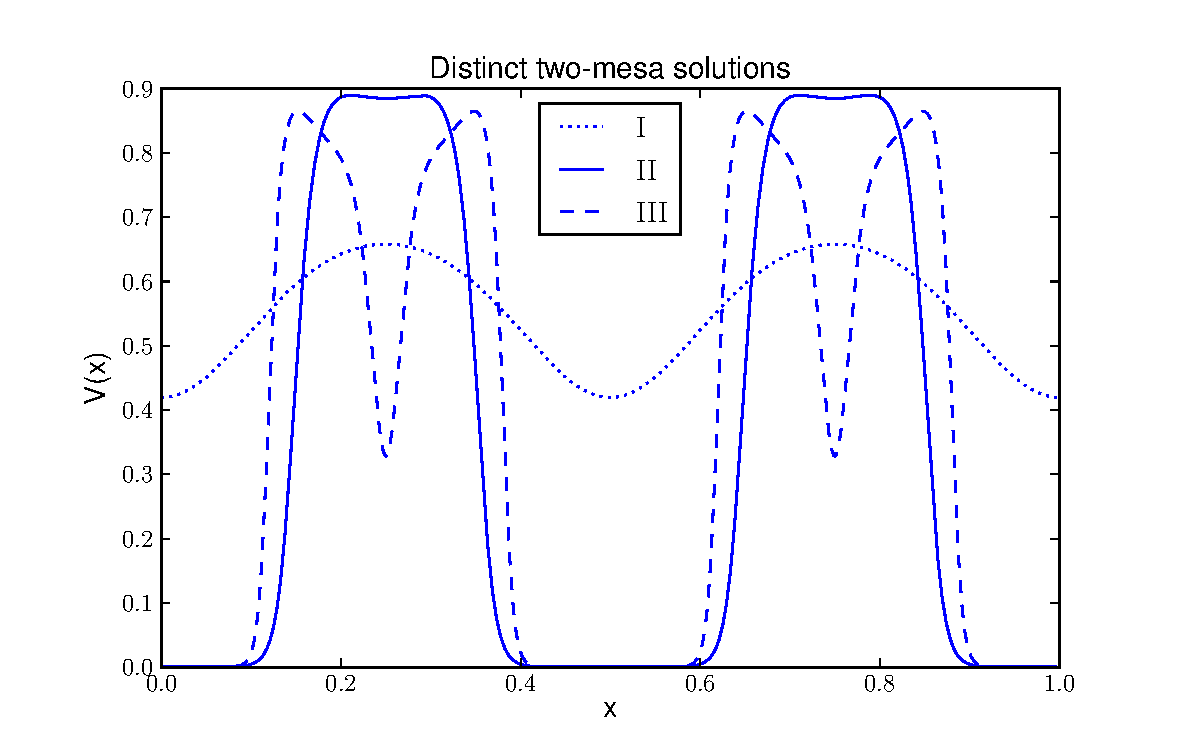
\includegraphics[width=2.5in]{typical_solutions}\includegraphics[width=2.5in]{two_mesa_branch}

\caption{Three distinct 2-mesa solutions to the GMS system. Solution $I$ is close to the Turing instability, $II$ is the stable mesa solution, and $III$ is the unstable solution that develops when the domain length is increased past a critical point. The image on the right is the bifurcation diagram for the branch of two-mesa solutions.}
\label{fig:typical}
\end{center}
\end{figure}
% 
The three solutions all occur for varying values of the domain length. They were all obtained through numerical continuation on the $L$ parameter. We started by obtaining a stationary solution from random initial data, and from it we used the numerical continuation package AUTO-07P \cite{doedel_auto-07p} to follow the curve of solutions for varying $L$, using $max(V)$ as the bifurcation parameter. 

Solution $I$ is essentially the leading eigenvector $\phi = A\cos(2n\pi x/L)$, first estimated through linear stability analysis, and as expected from Turing theory, unstable. Going up on the branch beyond solution $I$ leads to the homogeneous Turing solution $u=0.5603$, $v=u^2$, and traversing the branch in the other direction leads to the stable mesa branch.

Solution $II$ corresponds to the stable family of solutions, this is a characteristic mesa structure. Increasing $L$ and continuing on the branch eventually leads to a fold point, beyond which we reach the unstable branch characterized by solution $III$. Going beyond the fold point causes the solution to drop to the next branch of solutions, which will have double the number of mesas.

*****aqui me quede, 22jul

% 
\begin{figure}[htb]
\begin{center}
\includegraphics[width=3.5in]{one_sol_bif}
\caption{Four branches of the GMS system, with an overlay of the family of stable solutions obtained by traversing it left to right . When reaching the fold point of each branch the solutions fall to the next branch, effectively doubling the number of mesas. The upper horizontal unstable line are the unstable Turing solutions, and the red points on it are the values shown on table \ref{tab:L_turing}.}
\label{fig:one_sol}
\end{center}
\end{figure}
% 

The bifurcation diagram for one, two, four, and eight mesa solutions is given in figure \ref{fig:one_sol}. The thickest line is a stable solution that is recomputed for increasing values of $L$. It traverses the stable branches from left to right, and at each fold point it falls to the next branch, which manifests in the solutions as a doubling in the number of mesas. Since each successive branch doubles the number of mesas, the critical value $L_c$ at which the new set of mesas will split doubles with each iteration, hence $L_c(n)=L_c(1)\times 2^n$. This exponential relationship can be readily seen in the bifurcation diagram of figure \ref{fig:one_sol}, which was plotted on a logarithmic scale.

Furthermore, the system exhibits hysteresis, traversing the bifurcation diagram left to right produces a very different picture. Traversing left to right shows the splittings occurring at the points predicted in \eqref{eqn:final1}, whereas traversing in the opposite direction results in in the solution staying in the 8-mesa branch from $L=18$ up to $L~2.5$, beyond which the solution will jump either to the 4-mesa branch, or to the 2-mesa branch (very sensitive???). Two figures with the solution for $v(x)$ when traversed in either direction are shown in figure \ref{fig:up_down}.

% 
\begin{figure}[htb]
\begin{center}
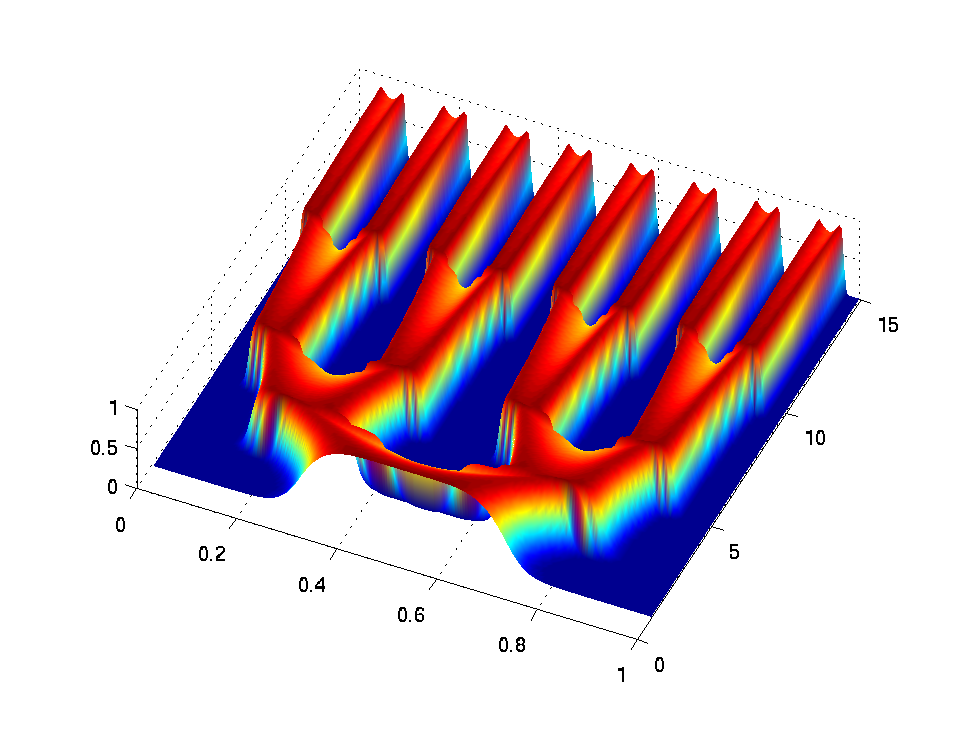
\includegraphics[width=2.5in]{full_soln_up}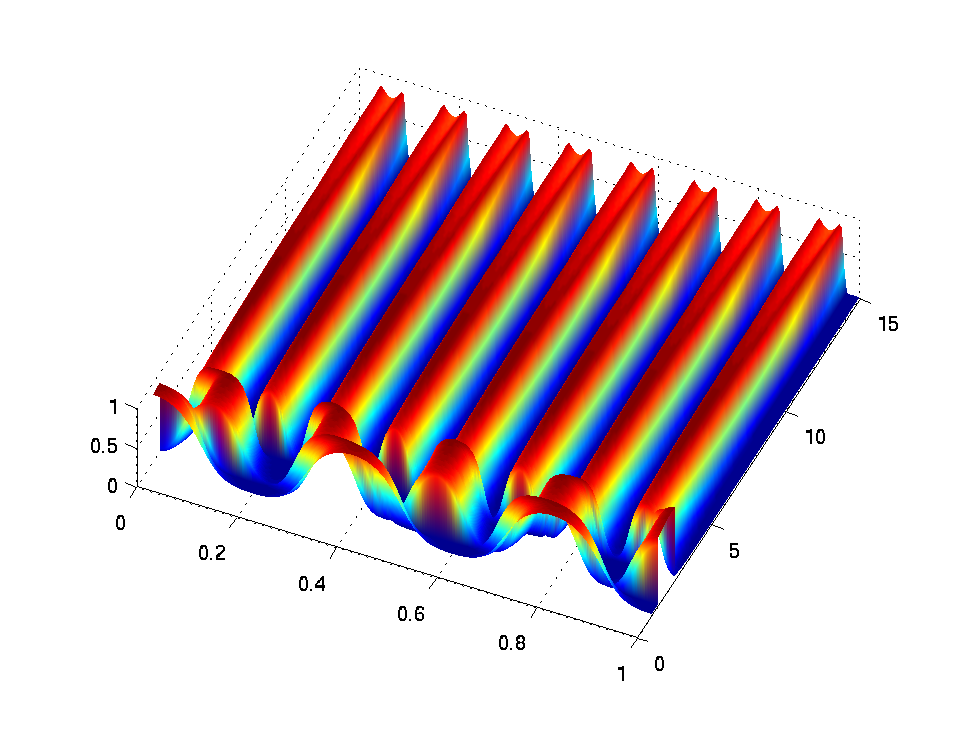
\includegraphics[width=2.5in]{full_soln_down}
\caption{The full solution curve for $v(x)$ as $L$ is varied from left to right (image on the left), and from right to left (image on the right).}
\label{fig:up_down}
\end{center}
\end{figure}
% 

We had previously derived an asymptotic formula in \eqref{eqn:final1} that estimates the critical value $L_c$ at which a one-mesa solution splits into two. In order to numerically compute the value, we first found the $u_c$, $v_c$ values that satisfy the Maxwell line condition, shown in \eqref{eqn:maxwell}, via a quadrature. It was then straightforward to numerically integrate $F(u_c;u_0)$ and the third term in \eqref{eqn:final1}. 

The resulting value was $L_c = 2.1010$ for $-L<x<L$, or half that for $0<x<L$ (as shown in figures \ref{fig:one_sol}, \ref{fig:typical}, \ref{fig:up_down}). The location of the fold point in the 1-mesa branch was then calculated by solving the full system, using $\Ep=0.002$ and $1500$ grid points. The value thus obtained was $L_c = 2.1325$.


\subsection{Construction of the solution in the near-shadow limit}

For the near-shadow limit, $D=\DD/\Ep$, we want to construct a $K-$stripe stationary solution on $x\in[0,1]$, with $L=1/K$ the period of the solution, and $l$ the length of each individual mesa, as shown in Figure \eqref{fig:single_mesa}.
% 
\begin{figure}[htb]
\begin{center}
\includegraphics[width=4in]{single_mesa}
\caption{A typical mesa profile in the stationary solution $v(x)$. The left and right edges of the mesa are labelled as $\chi_l$ and $\chi_r$ respectively; and the length of the mesa section is $l$.}
\label{fig:single_mesa}
\end{center}
\end{figure}
% 
The stationary equation we want to solve is
% 
\begin{equation}
\label{eqn:o-gms_stat}
\begin{split}
\begin{aligned}
	0 &= \Ep^2 u_{xx} -u + \frac{u^2}{v(1+ku^2)},\qquad &u_x(0)=u_x(L)=0, \\
	0 &= \frac{\DD}{\Ep}v_{xx} - v + u^2,\qquad &v_x(0)=v_x(L)=0.
\end{aligned}
\end{split}
\end{equation}
% 

***did not define $g(u,v)=\frac{u^2}{v(1+ku^2)}$, as it's only used much further down the road***

To first order, we have in the $v$ equation that $v_{xx}=0$. Applying the Neumann condition, we have then that $v\sim\VV$, and the value of the constant can be estimated by integrating over the whole domain,
% 
\begin{equation}
\label{eqn:o-v_first_order}
  \VV = \frac{1}{L}\int_0^Lu^2dx.
\end{equation}
% 

In the inner region near the left boundary of the mesa we have that $v=\VV$, and we do a change of variables for $u=\VV w$ and $y=\Ep^{-1}(x-\chi_l)$. The resulting equation is
% 
\begin{equation}
\label{eqn:o-w_eqn}
  w_{yy}+f(w)=0, \qquad -\infty<y<\infty,\qquad f(w) = -w + \frac{w^2}{1+bw^2},
\end{equation}
% 
with $b = k\VV^2$. Now, we are looking for a heteroclinic connection in $u$ as the transition mechanism that generates the mesa, one for the each side of the mesa. For a heteroclinic connection to exist in \eqref{eqn:o-w_eqn}, it has to satisfy the Maxwell line condition \cite{maxwell1994}.
% 
\begin{figure}[htb]
\begin{center}
\includegraphics[width=4in]{f_of_w}
\caption{A plot of the function $f(w)$ given in \eqref{eqn:o-w_eqn}.}
\label{fig:f(w)}
\end{center}
\end{figure}
% 

The function $f(w)=0$ has zeros at $w=0$ and $w_{\pm} = \frac{1\pm\sqrt{1-4b}}{2}$, with distinct real values for $w_{\pm}$ existing in the range $0\le b<1/4$. The profile of the curve in that range can be seen in Figure \eqref{fig:f(w)}. The Maxwell line condition states that a heteroclinic connection will exist for the value $b=b_0$ such that $\int_0^{w_+} f(w)dw = 0$. Integrating $f(w)$ we get
% 
\begin{equation*}
% \label{eqn:maxwell_lc}
\begin{split}
\begin{aligned}
  \int_0^{w_+} f(w)dw &= \left.\left(-\frac{w^2}{2} + \frac{w}{b} - \frac{1}{b^{3/2}}\arctan(b^{1/2}w) \right)\right|_0^{w_+},\\
  & = -\frac{w_+^2}{2} + \frac{w_+}{b_0} - \frac{1}{b_0^{3/2}}\arctan(b_0^{1/2}w_+),
\end{aligned}
\end{split}
\end{equation*}
% 
and since we have that $b_0 = \frac{w_+-1}{w_+^2}$, the Maxwell line condition will be satisfied if
% 
\begin{equation}
\label{eqn:maxwell2}
b_0 = \frac{w_+-1}{w_+^2},\qquad \sqrt{w_+-1}(w_++1)=2w_+\arctan(\sqrt{w_+-1}).
\end{equation}

This can be solved numerically to obtain the critical values $b_0 = 0.211376$, and $w_+ = 3.295209$. (??? do a plot of numerical vs asymptotic approximation)

For use later in section \eqref{section:stability}, we need to compute
% 
$$
\beta = \int_{-\infty}^{\infty}w'^2dy
$$
% 

We multiply \eqref{eqn:o-w_eqn} by $w'$ to get 
% 
\begin{equation*}
  \frac{d}{dy}\left(\frac{w'^2}{2} \right)=\frac{d}{dy}\mathcal{F}(w)\qquad\rightarrow\qquad w'^2 = 2\mathcal{F},
\end{equation*}
% 
with $\mathcal{F} = \int_0^wf(s)ds$. We then get
% 
\begin{equation}
\label{eqn:o-beta}
  \beta = \int_{-\infty}^{\infty}w'^2dy = \int_{0}^{w_+}w'^2\frac{1}{w'} dw = \int_{0}^{w_+}\sqrt{2\mathcal{F}(w)}dw.
\end{equation}
% 

This can be numerically calculated using the previously computed value for $w_+$, to get $\beta\sim1.49882$.

Linearizing around $w=0$ for $y\rightarrow -\infty$, and for $w=w_+$ for $y\rightarrow \infty$, we get that for $b=b_0$ we have a heteroclinic solution 
% 
\begin{equation*}
% \label{eqn:hetero}
\begin{split}
\begin{aligned}
  &w''+f(w)=0,\qquad &-\infty<y&<\infty,\qquad f(w) = -w + \frac{w^2}{1+b_0w^2},\\
  &w\sim d_-e^y,\qquad &&\mathrm{as}\hspace{2pt}y\rightarrow -\infty,\\
  &w\sim w_+ - d_+e^{-\nu_+y},\qquad&&\mathrm{as}\hspace{2pt}y\rightarrow \infty,
\end{aligned}
\end{split}
\end{equation*}
% 
for $\nu_+ = \sqrt{1-2/w_+}$. By translation we take $w(0)=w_+/2$, in order to have uniqueness.

A full mesa solution will consist of two back-to-back heteroclinic curves, and can be constructed as
% 
\begin{equation*}
  u\sim \VV[w_l + w_r - w_+],\qquad  \textrm{with }w_l\sim w\left(\frac{x-\chi_l}{\Ep}\right),\qquad w_r\sim w\left(\frac{\chi_r-x}{\Ep}\right).
\end{equation*}
% 

Integrating \eqref{eqn:o-v_first_order}, we get that to first order $\VV\sim\frac{1}{L}\VV^2w_+^2l$, with $l=\chi_r-\chi_r$ the width of the mesa. We then have
% 
\begin{equation*}
  \VV w_+^2\sim\frac{L}{l} + O(\Ep),\qquad l\sim\frac{L\sqrt{k}}{\sqrt{b_0}w_+^2}<L,
\end{equation*}
% 
therefore a necessary condition for a $K-$stripe solution to exist is that 
% 
\begin{equation*}
  \frac{\sqrt{k}}{\sqrt{b_0}w_+^2}<1.
\end{equation*}
% 

To refine the solution, it is necessary to further expand $u(x)$ and $v(x)$. In the outer region we expand $u$ and $v$ as
$$
v\sim \VV + \Ep v_1 + \Ep^2 h_2 + \cdots.
$$

Since outside of the mesa $u$ is exponentially small, and in the plateau region $u\sim\VV w_+ + O(\Ep)$, by substituting into \eqref{eqn:o-gms_stat}, we get that
% 
\begin{equation}
\label{eqn:o-v1}
	\begin{split}
	\DD v_{1,xx}
   = \left\{
	\begin{matrix}
		\VV& \mathrm{for}\hspace{2pt}0< x<\chi_l \\
		\VV(1-\VV w_+^2) = \VV(1-L/l)& \mathrm{for}\hspace{2pt}\chi_l< x<\chi_r\\
		\VV& \mathrm{for}\hspace{2pt}\chi_r<x<L
	\end{matrix}\right.
	\end{split}
\end{equation}
% 
with $v_{1,x}(0) = v_{1,x}(L) = 0$. In order to find the conditions on $v_1$ at the transition layers $\chi_l$ and $\chi_r$, we expand $u$ as $u\sim\VV w_+ + \Ep\UU_1 + ...$ on $\chi_l<x<\chi_r$.

Substituting into \eqref{eqn:o-gms_stat}, we get that 
\[
-\UU_1 + g_u(\VV w_+,\VV)\UU_1 + g_v(\VV w_+,\VV)v_1 = 0.
\]

Since $1+b_0w_+^2 = w_+$, the linearization terms simplify to
% 
\begin{equation}
\label{eqn:derivs}
\begin{split}
\begin{aligned}
  g_u(\VV w_+,\VV) = \frac{2w_+}{(1+b_0w_+^2)^2} = \frac{2}{w_+},\\
  g_v(\VV w_+,\VV) = \frac{-w_+^2}{1+b_0w_+^2} = -w_+,
\end{aligned}
\end{split}
\end{equation}
% 
and this yields
$$
-\UU_1 + \frac{2}{w_+}\UU_1 - w_+v_1 = 0,\qquad \Rightarrow \qquad \UU_1 = \frac{w_+^2}{2-w_+}v_1.
$$

We now expand $u$ and $v$ near the $x=\chi_l$ $(y=\Ep^{-1}(x-\chi_l))$ as
% 
\begin{equation*}
  u = u_0 + \Ep u_1 + \Ep^2 u_2+ \cdots,\qquad v = \VV + \Ep\VV_1 + \Ep^2\VV_2+\cdots,
\end{equation*}
% 
with $u_0 = \VV w_+$. Substituting into \eqref{eqn:o-gms_stat}, the $O(\Ep)$ system is
% 
\begin{equation}
\label{eqn:ord_epsilon}
\begin{split}
\begin{aligned}
  \LL u_1:&\equiv u_1''-u_1 + g_u(u_0,\VV)u_1 = -g_v(u_0,\VV)\VV_1 \\
  \VV_1'' &= 0.
\end{aligned}
\end{split}
\end{equation}
% 

For $\VV_1$ we get that $\VV_1 = \VV_{10} + \VV_{11}y$. We have that $\LL a_0' = 0$.

The solvability condition on \eqref{eqn:ord_epsilon} is then that 
% 
\begin{equation}
\label{eqn:solvab}
\begin{split}
\begin{aligned}
\int_{-\infty}^{\infty}g_v(u_0,\VV)\VV_1u_0'dy = \int_{-\infty}^{\infty}\frac{w^2}{1+bw^2}w'\VV_1dy = 0.
\end{aligned}
\end{split}
\end{equation}
% 

Substituting in $\VV_1 = \VV_{10} + \VV_{11}y$, the condition from \eqref{eqn:solvab} implies that
% 
\begin{equation*}
% \label{eqn:solvab2}
\begin{split}
\begin{aligned}
\VV_{10}\int_{-\infty}^{\infty}\frac{w^2w'}{1+bw^2}dy + \VV_{11}\int_{-\infty}^{\infty}\frac{w^2w'y}{1+bw^2}dy = 0.
\end{aligned}
\end{split}
\end{equation*}
% 

Since $\VV_1 = O(\Ep)$, $\VV_{11}$ has to be zero, as otherwise for $|y|\gg 1$ we would have $\VV_1 = O(1)$. Consequently, $\VV_{10}$ also has to be zero, and the conclusion is that $\VV_1=0$. We have then that $\LL u_1 = 0$, and therefore we also have $u_1 = 0$

This result yields that 
% 
\begin{equation*}
  v_1(\chi_l)  = v_1(\chi_r) = 0,
\end{equation*}
% 
and now we have enough conditions to solve uniquely for $v_1$.

Using the fact that $\chi_r-\chi_l = l$, and that $\VV w_+^2 = L/l$, the full solution to \eqref{eqn:o-v1} is
% 
\begin{equation*}
% \label{eqn:v1_full}
	\begin{split}
	v_1
   = \left\{
	\begin{matrix}
		\frac{\VV}{2\DD}(x^2-\chi_l^2)& \mathrm{for}\hspace{2pt}0< x<\chi_l \\
		\frac{\VV(l-L)}{2\DD l}[(x-\chi_l)^2 - l(x-\chi_l)]& \mathrm{for}\hspace{2pt}\chi_l< x<\chi_r\\
		\frac{\VV}{2\DD}[(L-x)^2-(L-\chi_r)^2]& \mathrm{for}\hspace{2pt}\chi_r<x<L
	\end{matrix}\right.
	\end{split}
\end{equation*}
% 

It is possible now to calculate $v_{1,x}$ close to the transition layers. We have
% 
\begin{equation}
\label{eqn:v1x}
\begin{split}
\begin{aligned}
  v_{1,x}(\chi_l^-) = \frac{\VV\chi_l}{\DD},\qquad &v_{1,x}(\chi_l^+) = \frac{\VV(L-l)}{2\DD},\\
  v_{1,x}(\chi_r^-) = -\frac{\VV(L-l)}{2\DD},\qquad &v_{1,x}(\chi_r^+) = -\frac{\VV(L-\chi_r)}{\DD},\\
\end{aligned}
\end{split}
\end{equation}
% 

% From equilibrium theory (ref ???), we have that $v_{1,x}(\chi_l^-) = v_{1,x}(\chi_l^+)$, as well as $v_{1,x}(\chi_r^-) = v_{1,x}(\chi_r^+)$. This yields that $\chi_l = \frac{L-l}{2}$, and $\chi_r = \frac{L+l}{2}$.

This suggests that there is a term to next order, as $\VV_2\sim v_{1,x}(\chi_l)$. Expanding to next order in the inner region, as $u = u_0 + \Ep^2u_2$ and $v = \VV + \Ep^2\VV_2$, and defining $g_0(w) = \frac{w^2}{1+b_0w^2}$, we have the system
% 
\begin{equation*}
% \label{eqn:solva2}
\begin{split}
\begin{aligned}
  \LL u_2 =  u_2'' - u_2 + g_0'(w)u_2 = g_0(w)\VV_2,\\
  \VV_2'' = 0.
\end{aligned}
\end{split}
\end{equation*}
% 

We have then that $\VV_2 = \VV_{20} + y\VV_{21}$. 

We can derive a solvability condition from $\LL u_2 = g_0(w)\VV_2$, since $\LL w'=0$. We get
% 
\begin{equation*}
  \int_{-\infty}^{\infty}\VV_2g_0(w)w'dy = \int_{-\infty}^{\infty}(\VV_{20} + y\VV_{21})g_0(w)w'dy = 0,
\end{equation*}
% 

We can now match the inner solution to the outer solution evaluated at the interface, to determine $\VV_{20}$ and $\VV_{21}$. We get that
% 
\begin{equation*}
  \VV + \Ep^2(\VV_{20} + y\VV_{21}) + \cdots = \VV + \Ep v_1(\chi_l) + \Ep v_{1,x}(\chi_l^-)(x-\chi_l) + \Ep^2v_2(\chi_l)+\cdots
\end{equation*}
% 

From this we can conclude that $\VV_{21} = v_{1,x}(\chi_l^-)$, and that $\VV_{20} = v_2(\chi_l)$. This last value, for both the inner and outer solutions, can be calculated from the solvability condition given that we now know $\VV_{21}$. 

Furthermore, repeating the matching procedure with $x\rightarrow \chi_l^+$ yields the same value, as the outer solution has no ambiguity. From this we get that $v_{1,x}(\chi_l^+) = v_{1,x}(\chi_l^-)$. Repeating the procedure yet again at the right boundary $\chi_r$, we get the same result, i.e., $v_{1,x}(\chi_r^+) = v_{1,x}(\chi_r^-)$. Since we already knew from \eqref{eqn:v1x} that $v_{1,x}(\chi_l^+) = - v_{1,x}(\chi_r^-)$, we can solve for $\chi_l$ and $\chi_r$ to get that the position of the boundaries of the mesa on $[0,L]$ are
% 
$$
  \chi_l = \frac{L-l}{2}, \qquad \chi_r = \frac{L+l}{2},
$$
% 
with $l$ the length of the plateau. A corollary from this result is that that stationary mesa solutions have to be centred.

We can find a second solvability condition that will be of use later on. Differentiating with respect to $y$, we have
% 
\begin{equation*}
  \LL u_2' = -g_0''(w)u_2w' + g_0(w)\VV_2' + g_0'(w)\VV_2w',
\end{equation*}
% 
and using the fact that $\LL w'=0$, the solvability condition we get is
% 
\begin{equation}
\label{eqn:solva1}
\begin{split}
\begin{aligned}
  -\VV_{21}\int_{-\infty}^{\infty}g_0(w)w'dy = \int_{-\infty}^{\infty}(g_0'(w)\VV_2 - g_0''(w)u_2)w'^2dy,\\
  v_{1,x}(\chi_r)\int_{-\infty}^{\infty}g_0(w)w'dy = \int_{-\infty}^{\infty}(g_0'(w)\VV_2 - g_0''(w)u_2)w'^2dy,
\end{aligned}
\end{split}
\end{equation}
% 
since $\VV_2' = \VV_{21} = -v_{1,x}(\chi_r)$.


\subsection{\label{section:stability}Stability in the near-shadow limit to perturbations in the y direction}

We assume that the solutions exist in a rectangular domain $[0,1]\times[0,d_0]$, with Neumann boundary conditions on all sides. We introduce a perturbation on the equilibrium solution $(u_e,v_e)$ of the form
% 
\begin{equation*}
  u = u_e + e^{\lA timy}\phi(x),\qquad v = v_e + e^{\lA timy}\psi(x); \qquad m = \frac{k\pi}{d_0},k=1,2,\ldots,
\end{equation*}
%
with $|\phi(x)|\ll1$, and $|\psi(x)|\ll1$.

Substituting into \eqref{eqn:o-gms1}, we get the following eigenvalue problem
%
\begin{subequations}
\begin{align}
\label{eqn:eigen_gms1}
  \bar{\lA}\phi = \LL_{\Ep}\phi + g_v(u_e,v_e)\psi &= \Ep^2\phi_{xx} - \phi + g_u(u_e,v_e)\phi + g_v(u_e,v_e)\psi,\\
\label{eqn:eigen_gms2}
  \frac{\Ep}{\DD}(1+\tau\lA)\psi &= \psi_{xx} - m^2\psi + \frac{2\Ep}{\DD}u_e\phi,
\end{align}
\end{subequations}
% 
with $\bar{\lA} = \lA + \Ep^2m^2$, and Neumann conditions $\phi_x(0)=\phi_x(1)=\psi_x(0)=\psi_x(1)=0$.

As shown in \eqref{eqn:derivs}, in the plateau region we have that $g_u(u_e,v_e) = 2/w_+$, and $g_v(u_e,v_e) = -w_+$. Substituting into \eqref{eqn:eigen_gms1}, we have that, to first order, when $\bar{\lA}\ll 1$ (???), the asymptotic form of $\phi$ on the plateau region is 
% 
\begin{equation*}
  \phi = \mu\psi,\qquad \textrm{with  }\mu \equiv \frac{w_+^2}{2-w_+},\qquad \chi_l<x<\chi_r.
\end{equation*}
% 
Outside of the plateau region $\phi$ is asymptotically small, therefore near the transition layers located at $\chi_l,\chi_r$, $\phi$ is proportional to the derivative $w'$ of the heteroclinic connection. We have then the following asymptotic form for $\phi$
% 
\begin{equation*}
% \label{eqn:phi_asy2}
	\begin{split}
	\phi
   \sim \left\{
	\begin{matrix}
		c_{li}(w'(\Ep^{-1}(x-\chi_{li}))+O(\Ep))& \mathrm{for}\hspace{2pt} x\sim\chi_{li}& \\
		c_{ri}(w'(\Ep^{-1}(\chi_{ri}-x))+O(\Ep))& \mathrm{for}\hspace{2pt} x\sim\chi_{ri}& \\
		\phi_i = \mu\psi& \mathrm{for}\hspace{2pt}x\in(\chi_{li},\chi_{ri}),&i=1,\hdots,K,
	\end{matrix}\right.
	\end{split}
\end{equation*}
% 
with the constants $c_{li},c_{ri}$ to be found.

Since $\phi$ is localized near the transition layers, we can estimate it in the sense of distributions, approximating $u_e$ as $u_e\sim\VV w$
% 
\begin{equation*}
\begin{split}
\begin{aligned}
  \frac{2\Ep u_e\phi}{\DD}&\sim \frac{2\Ep^2\VV c_l}{\DD}\int_{-\infty}^{\infty}w_lw_l'dy\dE(x-x_l) +...\\ 
  &\qquad+\frac{2\Ep^2\VV c_r}{\DD}\int_{-\infty}^{\infty}w_rw_r'dy\dE(x-x_r) + \frac{2\Ep\VV}{\DD}w_+\mu\psi H_{[\chi_l,\chi_r]},
\end{aligned}
\end{split}
\end{equation*}
% 
with $H_{[\chi_l,\chi_r]} = 1$ on $x\in (\chi_l,\chi_r)$, and zero elsewhere.

This then yields
% 
\begin{equation*}
% \label{eqn:phi_main}
\begin{split}
\begin{aligned}
\frac{2\Ep u_e\phi}{\DD}&\sim \frac{\Ep^2\VV c_lw_+^2}{\DD}\dE(x-x_l) +\frac{\Ep^2\VV c_rw_+^2}{\DD}\dE(x-x_r) + \frac{2\Ep\VV w_+\mu\psi H}{\DD}
\end{aligned}
\end{split}
\end{equation*}
% 
Substituting into \eqref{eqn:eigen_gms2}, we get that $\psi$ satisfies
% 
\begin{equation}
\label{eqn:phi_main2}
\begin{split}
\begin{aligned}
\psi_{xx}-\tH^2\psi = -\frac{\Ep^2\VV w_+^2}{\DD}\left[\sum_i(c_{li}\dE(x-\chi_{li}) + c_{ri}\dE(x-\chi_{ri})) \right],
\end{aligned}
\end{split}
\end{equation}
% 
with $\tH$ the piecewise constant function
% 
\begin{equation}
\label{eqn:phi_asym}
	\begin{split}
	\tH
   = \left\{
	\begin{matrix}
		\tH_-\equiv\left(m^2+\frac{\Ep(1+\tau\lA)}{\DD}\right)^{1/2},& \mathrm{for}\hspace{2pt} x\notin\cup_{i=1}^K[\chi_{li},\chi_{ri}]\\
		\tH_+\equiv\left(m^2+\frac{\Ep(1+\tau\lA)}{\DD}\left(1+\frac{2w_+}{l(w_+-2)} \right)\right)^{1/2},& \mathrm{for}\hspace{2pt} x\in\cup_{i=1}^K[\chi_{li},\chi_{ri}]
	\end{matrix}\right.
	\end{split}
\end{equation}
% 

Since $w'$ is localized, we can define $w'_{li}=w'(x-\chi_{li})$ and $w'_{ri}=w'(\chi_{ri}-x)$, and multiply it into \eqref{eqn:eigen_gms1}, to obtain the matrix eigenvalue problem
% 
\begin{equation}
\label{eqn:matrix_eigen_l}
  c_{li}(w'_{li},\LL_{\Ep}w'_{li}) + (w'_{li},g_v(u_e,v_e)\psi) = c_{li}\bar{\lA}(w'_{li},w'_{li}),
\end{equation}
% 
and similarly
% 
\begin{equation}
\label{eqn:matrix_eigen_r}
  c_{ri}(w'_{ri},\LL_{\Ep}w'_{ri}) + (w'_{ri},g_v(u_e,v_e)\psi) = c_{ri}\bar{\lA}(w'_{ri},w'_{ri}),
\end{equation}
% 
where $(f,g) = \int_0^1fgdx$.

The second term in \eqref{eqn:matrix_eigen_l} and \eqref{eqn:matrix_eigen_r} can be readily estimated, using the fact that $w''-w = g_0(w)$, and that $g_v=-g_0$, as
% 
\begin{equation*}
\begin{split}
\begin{aligned}
% \label{eqn:2ndterml}
  (w'_{li},g_v(u_e,v_e)\psi) = \int_0^1 w_{li}'\psi g_v(u_e,v_e)dx  =-\Ep\psi(\chi_l)\int_{-\infty}^{\infty}w'g_0(w)dy  \\
  =-\Ep\psi(\chi_l)\int_{-\infty}^{\infty}w'(w''-w)dy = -\Ep\psi(\chi_l)\frac{w_+^2}{2},
\end{aligned}
\end{split}
\end{equation*}
% 
and similarly, 
% 
\begin{equation*}
\begin{split}
\begin{aligned}
% \label{eqn:2ndtermr}
  (w'_{ri},g_h(u_e,v_e)\psi) = -\Ep\psi(\chi_r)\frac{w_+^2}{2}.
\end{aligned}
\end{split}
\end{equation*}
% 

The third term can be estimated straight from the definition of $\beta$ in \eqref{eqn:o-beta}. We get
% 
\begin{equation*}
\begin{split}
\begin{aligned}
% \label{eqn:third term}
  (w'_{li},w'_{li})) \sim \Ep\int_{-\infty}^{\infty}(w')^2dy = \Ep\beta.
\end{aligned}
\end{split}
\end{equation*}
% 

The first term can be estimated using some of the results previously obtained. We have that 
% 
\begin{equation*}
  \LL_{\Ep}w_l'=(w_l')''-w_l'+g_u(u_e,v_e)w_l'.
\end{equation*}
%

We can approximate $g_u(u_e,v_e)$ as 
% 
\begin{equation*}
g_u(u_e,v_e)\sim g_u(w\VV,\VV) + \Ep^2(g_{uu}(w\VV,\VV) + g_{uv}(w\VV,\VV))+\cdots.
\end{equation*}
% 
The derivatives can be related to $g_0(w) = \frac{w^2}{1+b_0w^2}$ in the following way:
% 
\begin{equation*}
\begin{split}
\begin{aligned}
% \label{eqn:derivs_g}
  g_u(u,v)&=\frac{2u}{v(1+ku^2)^2}\sim\frac{2w}{(1+b_0w^2)^2}=g_0'(w),\\
  g_{uu}(u,v)&=\frac{1}{v}\frac{2-6ku^2}{(1+ku^2)^3}\sim\frac{1}{\VV}\frac{2-6b_0w^2}{(1+b_0w^2)^3}=\frac{1}{\VV}g_0''(w),\\
  g_{uv}(u,v)&=-\frac{2u}{v^2(1+ku^2)^2}\sim-\frac{2w}{\VV(1+b_0w^2)^2}=-\frac{1}{\VV}g_0'(w).
\end{aligned}
\end{split}
\end{equation*}
% 

Substituting them in, we get
% 
\begin{equation*}
\begin{split}
\begin{aligned}
  g_u(u_e,v_e)\sim g_0'(w)+\frac{\Ep^2}{\VV}(g_0''(w)u_2 - g_0'(w)\VV_2)+\cdots,\\
  \LL_{\Ep}w_{li}' \sim \frac{\Ep^2}{\VV}(g_0''(w_{li})u_2 - g_0'(w_{li})\VV_2)w_{li}'.
\end{aligned}
\end{split}
\end{equation*}
%

We then get for the first term
% 
\begin{equation*}
\begin{split}
\begin{aligned}
  (w'_{li},\LL_{\Ep}w'_{li}) &\sim \frac{\Ep^2}{\VV}\int_0^1\left(g_0''(w_{li})u_2 - g_0'(w_{li})\VV_2 \right)w_{li}'^2dx \\
  &\qquad= \frac{\Ep^3}{\VV}\int_{-\infty}^{\infty}\left(g_0''(w_{li})u_2 - g_0'(w_{li})\VV_2 \right)w_{li}'^2dy
\end{aligned}
\end{split}
\end{equation*}
% 

Using the solvability condition in \eqref{eqn:solva1}, 
% 
\begin{equation*}
\begin{split}
\begin{aligned}
  \VV_2'\int_{-\infty}^{\infty}g_0(w)w'dy = \int_{-\infty}^{\infty}(g_0'(w)\VV_2 - g_0''(w)u_2)w'^2dy,
\end{aligned}
\end{split}
\end{equation*}
% 
we get
% 
\begin{equation*}
\begin{split}
\begin{aligned}
  (w'_{li},\LL_{\Ep}w'_{li}) &\sim \frac{\Ep^3}{\VV}\VV_2'\int_{-\infty}^{\infty}g_0(w)w'dy = \frac{\Ep^3}{\VV}\VV_2'\int_{-\infty}^{\infty}(w-w'')w'dy\\
  &\qquad = \frac{\Ep^3\VV_2'}{2\VV}w_+^2 = \frac{\Ep^3v_{1x}(\chi_{li})w_+^2}{2\VV}
\end{aligned}
\end{split}
\end{equation*}
% 

Similarly, on the other side of the plateau the process is identical, except for a sign change in the slope,
% 
\begin{equation*}
\begin{split}
\begin{aligned}
  (w'_{ri},\LL_{\Ep}w'_{ri}) &\sim -\frac{\Ep^3v_{1x}(\chi_{ri})w_+^2}{2\VV}
\end{aligned}
\end{split}
\end{equation*}
% 

Putting everything together results in the following $2K\times 2K$ system
% 
\begin{equation*}
% \label{eqn:system0}
\begin{split}
\begin{aligned}
  \Ep\bar{\lA} c_{li}\beta &\sim \frac{\Ep^3}{2\VV}c_{li}v_{1x}(\chi_{li})w_+^2 - \frac{\Ep}{2}\psi(\chi_{li})w_+^2,\\
  \Ep\bar{\lA} c_{ri}\beta&\sim - \frac{\Ep^3}{2\VV}c_{ri}v_{1x}(\chi_{li})w_+^2 - \frac{\Ep}{2}\psi(\chi_{ri})w_+^2,
\end{aligned}
\end{split}
\end{equation*}
% 
and since from \eqref{eqn:v1x} we know that 
% 
\[
  v_{1x(\chi_{li})} = \frac{\VV(L-l)}{2\DD},
\]
% 
the above system can be simplified to 
% 
\begin{equation}
\label{eqn:system1}
\begin{split}
\begin{aligned}
  \bar{\lA}\beta c_{li} &\sim \Ep^2\frac{(L-l)w_+^2}{4\DD}c_{li} - \frac{w_+^2}{2}\psi(\chi_{li}),\\
  \bar{\lA}\beta c_{ri}&\sim - \Ep^2\frac{(L-l)w_+^2}{4\DD}c_{ri} - \frac{w_+^2}{2}\psi(\chi_{ri}).
\end{aligned}
\end{split}
\end{equation}
% 

This equation, together with \eqref{eqn:phi_main2} constitutes a system for $\bar\lA$ and $\vec{c} = [c_{li},c_{ri}]$. 

The system given in \eqref{eqn:system1} depends on $\psi(\chi_{ri})$ and $\psi(\chi_{li})$. Solving \eqref{eqn:phi_main2} explicitly, we get
% 
\begin{equation}
\label{eqn:psi_soln}
	\begin{split}
	\psi(x)
   = \left\{
	\begin{matrix}
		\psi_{l1}\cosh(\tH_-x),& \text{for  }0<x<\chi_{l1}\\
		\psi_{li}\cosh(\tH_+(x-\chi_{li})) + B_{li}\sinh(\tH_+(x-\chi_{li})),& \text{for  }\chi_{li}<x<\chi_{ri}\\
		\psi_{ri}\cosh(\tH_-(x-\chi_{ri})) + B_{di}\sinh(\tH_-(x-\chi_{ri})),& \text{for  }\chi_{ri}<x<\chi_{l(i+1)}\\
		\psi_{lK}\cosh(\tH_-(x-1)),& \text{for  }\chi_{rK}<x<1
	\end{matrix}\right.
	\end{split}
\end{equation}
% 
for $i=2,\ldots,K-1$, where $\psi_{li}\equiv \psi(\chi_{li}), \psi_{ri}\equiv \psi(\chi_{ri})$, and $B_{li},B_{di}$ have yet to be found. We have that $\chi_{ri} - \chi_{li} = l$; similarly, if we define $d\equiv\chi_{l(i+1)} - \chi_{ri} = \frac{1}{K} - l$, and the constants
% 
\begin{equation*}
\begin{split}
\begin{aligned}
  c_l = \cosh(\tH_+l),\qquad s_l = \sinh(\tH_+l),\\
  c_d = \cosh(\tH_-d),\qquad s_d = \sinh(\tH_-d)
\end{aligned}
\end{split}
\end{equation*}
% 
we have that $\psi_{ri} = \psi_{li}c_l + B_{li}s_l$, and that $\psi_{l(i+1)} = \psi_{ri} + B_{di}s_d$. This yields the following conditions
% 
\begin{equation*}
\begin{split}
\begin{aligned}
  B_{li} &= \frac{\psi_{ri} - \psi_{li}c_l}{s_l},\\
  B_{di} &= \frac{\psi_{l(i+1)} - \psi_{ri}c_d}{s_d}.\\
\end{aligned}
\end{split}
\end{equation*}
% 

Additionally, the jump condition that solution \eqref{eqn:psi_soln} has to satisfy is given by
% 
\begin{equation}
\label{eqn:jump_cond}
\begin{split}
\begin{aligned}
  -[\psi_x(\chi_{li}^+) - \psi_x(\chi_{li}^-)] &= \frac{\Ep^2\VV w_+^2}{\DD}c_{li} \equiv b_{li},\\
  -[\psi_x(\chi_{ri}^+) - \psi_x(\chi_{ri}^-)] &= \frac{\Ep^2\VV w_+^2}{\DD}c_{ri} \equiv b_{ri},
\end{aligned}
\end{split}
\end{equation}
% 
for $i=1,\ldots,K$. We then calculate $\psi_x$ from \eqref{eqn:psi_soln} to get
% 
\begin{equation*}
% \label{eqn:psi_eval}
\begin{split}
\begin{aligned}
  \psi_x(\chi_{li}^+) &= B_{li}\tH_+,\\
  \psi_x(\chi_{li}^-) &= \psi_{r(i-1)}\tH_-s_d + B_{d(i-1)}\tH_-c_d,\\
  \psi_x(\chi_{ri}^+) &= B_{di}\tH_-,\\
  \psi_x(\chi_{ri}^-) &= u_{li}\tH_+s_l + B_{li}\tH_+c_l.
\end{aligned}
\end{split}
\end{equation*}
% 

Substituting them into the jump condition yields
% 
\begin{equation*}
% \label{eqn:psi_eval_bl}
\begin{split}
\begin{aligned}
  b_{li} &= \psi_x(\chi_{li}^-) - \psi_x(\chi_{li}^+) = \psi_{r(i-1)}\tH_-s_d + B_{d(i-1)}\tH_-c_d -B_{li}\tH_+\\
		 &= \psi_{r(i-1)}\tH_-s_d + \left(\frac{\psi_{li} - \psi_{r(i-1)}c_d}{s_d}\right)\tH_-c_d -\left(\frac{\psi_{ri} - \psi_{li}c_l}{s_l}\right)\tH_+\\
		 &= \psi_{r(i-1)}\tH_-\left(s_d - \frac{c_d^2}{s_d} \right) - \psi_{ri}\frac{\tH_+}{s_l} + \psi_{li}\left(\tH_-\frac{c_d}{s_d} + \tH_+\frac{c_l}{s_l} \right)\\
		 &= - \psi_{r(i-1)}\frac{\tH_-}{s_d} - \psi_{ri}\frac{\tH_+}{s_l} + \psi_{li}\left(\tH_-\frac{c_d}{s_d} + \tH_+\frac{c_l}{s_l} \right),
\end{aligned}
\end{split}
\end{equation*}
% 
and similarly,
% 
\begin{equation*}
% \label{eqn:psi_eval_br}
\begin{split}
\begin{aligned}
  b_{ri} &= \psi_x(\chi_{ri}^-) - \psi_x(\chi_{ri}^+) = \psi_{li}\tH_+s_l + B_{li}\tH_+c_d -B_{di}\tH_-\\
		 &= - \psi_{l(i+1)}\frac{\tH_-}{s_d} - \psi_{li}\frac{\tH_+}{s_l} + \psi_{ri}\left(\tH_+\frac{c_l}{s_l} + \tH_-\frac{c_d}{s_d} \right),
\end{aligned}
\end{split}
\end{equation*}
% 
for $i=2,\ldots,K-1$. The values at the boundaries are slightly different and have to be derived separately,
% 
\begin{equation*}
\begin{split}
\begin{aligned}
  b_{l1} &= \psi_x(\chi_{l1}^-) - \psi_x(\chi_{l1}^+) = A_0\tH_-\sinh(\tH_-d/2) - B_{l1}\tH_+,\\
  b_{rK} &= \psi_x(\chi_{rK}^-) - \psi_x(\chi_{rK}^+) = A_K\tH_-\sinh(\tH_-d/2) + \psi_{lK}\tH_+s_l + B_{lK}\tH_+c_l.
\end{aligned}
\end{split}
\end{equation*}

Matching $\psi$ across $x=\chi_{l1}$ and $\chi_{rK}$ yields that $A_0 = \frac{\psi_{l1}}{\cosh(\tH_-d/2)}$, and similarly $A_K = \frac{\psi_{rK}}{\cosh(\tH_-d/2)}$. Using the identity
% 
\[
\frac{\sinh(x/2)}{\cosh(x/2)} = \frac{\cosh(x)-1}{\sinh(x)},
\]
% 
we finally have that 
% 
\begin{equation*}
% \label{eqn:psi_eval_b1K}
\begin{split}
\begin{aligned}
  b_{l1} &= \psi_{l1}\left(\tH_-\frac{c_d}{s_d} - \frac{\tH_-}{s_d} + \tH_+\frac{c_l}{s_l} \right) - \psi_{r1}\frac{\tH_+}{s_l}\\
  b_{rK} &= \psi_{rK}\left(\tH_-\frac{c_d}{s_d} - \frac{\tH_-}{s_d} + \tH_+\frac{c_l}{s_l} \right) - \psi_{lK}\frac{\tH_+}{s_l}.
\end{aligned}
\end{split}
\end{equation*}

We can now write the $2K\times2K$ system of equations in matrix form as $M\vec{\psi} = \vec{b}$, with $M$ the tridiagonal matrix
% 
\[
  M 
  = \left[
	\begin{matrix}
	  a+c & b \\
	  b & c & a \\
	  & a &c & b \\
	  & & & \ddots \\
	  & & & & b & c & a\\
	  & & & & & a & c & b\\
	  & & & & & & b & c + a\\
	\end{matrix}\right],
\]
% 
and where
% 
\[
  a = -\frac{\tH_-}{s_d},\qquad b = - \frac{\tH_+}{s_l},\qquad c = \frac{c_d}{s_d}\tH_-+\frac{c_l}{s_l}\tH_+.
\]

The eigenpairs of $M$ can be found explicitly (see appendix B in \cite{ren_spectra_2003}), and for the reader's convenience we will reproduce the calculation. (Probably put it in it's own appendix)

The $M$ matrix can be simplified into $M = Q + cI$, with 
% 
\[
  Q 
  = \left[
	\begin{matrix}
	  a & b \\
	  b & 0 & a \\
	  & a &0 & b \\
	  & & & \ddots \\
	  & & & & b & 0 & a\\
	  & & & & & a & 0 & b\\
	  & & & & & & b & a\\
	\end{matrix}\right].
\]
% 

We use the property that $\text{eig}(M) = c + \text{eig}(Q)$. We start by looking for an eigenvector $\vec{q} = [z,tz^2,z^3,tz^4,\hdots,tz^{2K}]^T$, with $t,z\in\mathbb{C}$, $|z|=1$, and corresponding eigenvalue $\sigma$. From the second equation to the second to last we get the following system,
% 
\begin{equation}
\label{eqn:eigen_Q}
\begin{split}
\begin{aligned}
  atz^{1-l}+btz^{1+l}=\sigma z^l,&\qquad \text{if  }l \text{  is odd},\\
  bz^{1-l}+az^{1+l}=\sigma tz^l,&\qquad \text{if  }l \text{  is even.}
\end{aligned}
\end{split}
\end{equation}
% 

Since $z\bar{z}=1$, hence $1/z = \bar{z}$, we can solve for $t$ in the above system to get
% 
\[
  t=\pm\frac{az+b\bar{z}}{|az+b\bar{z}|},
\]
% 
which implies that $|t|=1$.

In order to satisfy the first and last equations, we look at the extended system $Q(Ah+B\bar{h}) = \sigma (Ah+B\bar{h})$, with $h = [t,\vec{q},tz^{2K+1}]^T$. The first and last equations are
% 
\begin{equation*}
% \label{eqn:eigen_Q2}
\begin{split}
\begin{aligned}
  a(At+B\bar{t}) + b(Az+B\bar{z}) &= \sigma(At+B\bar{t}),\\
  b(Atz^{2K}+B\bar{t}\bar{z}^{2K}) + a(Az^{2K+1}+B\bar{z}^{2K+1}) &= \sigma(Az^{2K+1}+B\bar{z}^{2K+1}).
\end{aligned}
\end{split}
\end{equation*}
% 

The first and last equations will then be satisfied if
% 
\begin{equation*}
% \label{eqn:eigen_Q3}
\begin{split}
\begin{aligned}
  At+B\bar{t} &= Az+B\bar{z},\\
  Atz^{2K}+B\bar{t}\bar{z}^{2K} &= Az^{2K+1}+B\bar{z}^{2K+1}.
\end{aligned}
\end{split}
\end{equation*}
% 

Nontrivial solutions for $A$ and $B$ exist if 
% 
\[
  (z-t)(1-\bar{t}\bar{z})\bar{z}^{2K} = (\bar{z}-\bar{t})(1-tz)z^{2K}
\]
% 
is satisfied. Since $|z| = |t| = 1$, we have then that $z^{4K} = 1$. If we write $z$ in polar form, we have that the roots of $z^{4K} = 1$ are $z=e^{i\frac{2\pi(j-1)}{2K}}$, with $j=1,2,\hdots,2K$. Substituting it into \eqref{eqn:eigen_Q}, we get
% 
\[
  \sigma = \pm|az + b\bar{z}| = \pm\sqrt{a^2 + b^2 + 2ab\cos(\tH)},
\]
% 
with $\tH = \frac{2\pi(j-1)}{2K}$. Since we have both positive and negative values, we are counting twice when ranging $j=1,\hdots,2K$; therefore the range can be restricted to obtain the following set of distinct eigenvalues
% 
\begin{equation*}
% \label{eqn:eigen_Q4}
\begin{split}
\begin{aligned}
  \sigma_{j\pm} &= \pm\sqrt{a^2 + b^2 + 2ab\cos\tH_j},\qquad\text{with  }\tH_j=\frac{\pi j}{K},\qquad j=1,	\hdots,K-1,\\
  \sigma_{K\pm} &= a\pm b.
\end{aligned}
\end{split}
\end{equation*}

Going back to \eqref{eqn:jump_cond}, we can express the jump condition as the following system,
% 
\[
  \vec{\psi} = M^{-1}\vec{b} =\frac{\Ep^2\VV w_+^2}{D}M^{-1}\vec{c},
\]
% 
and we can use it to substitute $\vec{\psi}$ in \eqref{eqn:system1}, resulting in the system
%
\begin{equation}
\label{eqn:Kmesa_gms}
  \bar{\lA}\beta\vec{c} = \Ep^2\left(\frac{(L-l)w_+^2}{4\DD}I - \frac{\VV w_+^4}{2\DD}M^{-1}\right)\vec{c}.
\end{equation}
% 

Since $\bar{\lA} = \lA + \Ep^2m^2$, and $M^{-1}\vec{c} = \hat\sigma^{-1}\vec{c}$, with $\hat\sigma = c+\sigma$, we have then that in the limit when $\Ep\rightarrow 0$,
% 
\begin{equation*}
  \lim_{\Ep\rightarrow0}\frac{\lA_{j\pm}}{\Ep^2} = -m^2 + \frac{(L-l)w_+^2}{4\DD\beta} - \frac{\VV w_+^4}{2\DD\beta}\hat\sigma_{j\pm}^{-1},\qquad j=1,\hdots,K.
\end{equation*}

To establish the stability of the system, we want to establish conditions that guarantee that the eigenvalues will be negative, hence stable. 

The largest eigenvalue corresponds to the largest $\hat\sigma$ value; since both $a$ and $b$ are negative, the largest $\sigma$ values corresponds to $j=1$; and as the number of mesas increases the largest eigenvalue tends to $c+|a+b|$. 

On the other end of the spectrum, we have that the smallest eigenvalue is always positive,
% 
\[
  c+a+b = c-|a+b| = \frac{c_d\tH_-}{s_d}+\frac{c_l\tH_+}{s_l}-\frac{\tH_-}{s_d}-\frac{\tH_+}{s_l} = \frac{s_l\tH_-(c_d-1) + s_d\tH_+(c_l-1)}{s_ds_l},
\]
% 
since $\cosh(x)>1$ for $x\neq0$.

From \eqref{eqn:phi_asym} we have that to leading order both $\tH_-,\tH_+\sim m$. Let
% 
\[
 \hat{a} = \frac{-1}{\sinh(md)}, \qquad \hat{b} = \frac{-1}{\sinh(ml)},\qquad \hat{c} = \coth(md)+\coth(ml),
\]
% 
the stability condition is, then
% 
\begin{equation*}
% \label{eqn:stab_cond}
\begin{split}
\begin{aligned}
  \frac{(L-l)w_+^2}{4\DD\beta} &< m^2 + \frac{\VV w_+^4}{2\DD\beta}\hat\sigma_{j\pm}^{-1}\\
  &\qquad = m^2 + \frac{L w_+^2}{2\DD\beta lm}\left[\frac{1}{\hat{c}\pm \sqrt{\hat{a}^2+\hat{b}^2+2\hat{a}\hat{b}\cos\left(\frac{\pi j}{K}\right)}}\right],
\end{aligned}
\end{split}
\end{equation*}
% 
for all $j=1,\hdots,K-1$, and $m=\frac{k\pi}{d_0}$, $k=1,\hdots$.

A sufficient condition for stability is, then, that if
%
\begin{equation*}
 \DD > \frac{(L-l)w_+^2d_0^2}{4\pi^2\beta}
\end{equation*}
% 
then the $K-$stripe system will be stable.

For the $m=0$ mode, and to first order, we approximate $a$, $b$, and $c$ as
% 
\[
  a=-\frac{1}{d}+O(\Ep),\qquad b = -\frac{1}{l}+O(\Ep),\qquad c=\frac{1}{d}+\frac{1}{l}+O(\Ep),
\]
% 

Since $\hat\sigma_{K+}= a+b+c$ would be zero to first order, we can approximate $c$ to second order for that particular case, resulting in 
% 
\[
  c=\frac{1}{d}+\frac{1}{l}+\frac{1}{2}(d\tH_-^2+l\tH_+^2)+O(\Ep^2).
\]


We have then that
%
% \begin{subequations}
\[
\begin{align}
%  \label{eqn:sigmas}
  \hat\sigma_{j\pm} &\sim \frac{1}{d}+\frac{1}{l}\pm\sqrt{\frac{1}{d^2}+\frac{1}{l^2}+\frac{2}{dl}\cos(\tH_j)},\qquad j=1,\hdots,K-1,\\
  \hat\sigma_{K+} &\sim \frac{1}{2}(d\tH_-^2+l\tH_+^2),\\
  \hat\sigma_{K-} &\sim \frac{2}{l}.
\end{align}
% \end{subequations}
\]
% 

Similarly, we have that the eigenvalues $\lA_{j\pm}$ for the full system, for the $m=0$ mode, are
%
\begin{subequations}
\label{eqn:lambda_all}
% \begin{split}
\begin{align}
\label{eqn:lambda_all1}
  \lA_{K+} &= \Ep^2\left(\frac{(L-l)w_+^2}{4\DD\beta}-\frac{Lw_+^2}{2\DD\beta l}\sigma_{K+}^{-1} \right),\\
		  &= - \Ep\frac{Lw_+^2}{\beta l}\left[\frac{1}{K}-\frac{2w_+}{2-w_+}\right]^{-1} +O(\Ep^2)<0,\notag\\
\label{eqn:lambda_all2}
  \lA_{K-} &= \Ep^2\left(\frac{(L-l)w_+^2}{4\DD\beta}-\frac{Lw_+^2}{2\DD\beta l}\frac{l}{2}\right) = -\Ep^2\frac{lw_+^2}{4\DD\beta}<0,\\
\label{eqn:lambda_all3}
  \lA_{j\pm} &= \Ep^2\left(\frac{(L-l)w_+^2}{4\DD\beta}-\frac{Lw_+^2}{2\DD\beta l}\sigma_{j\pm}^{-1} \right),\qquad j=1,\hdots,K-1,\\
		  &<\Ep^2\left(\frac{(L-l)w_+^2}{4\DD\beta}-\frac{Lw_+^2}{2\DD\beta l}\left[\frac{2}{d}+\frac{2}{l}\right]^{-1} \right),\notag\\
		  &\qquad = \Ep^2\left(\frac{(L-l)w_+^2}{4\DD\beta}-\frac{Lw_+^2}{2\DD\beta l}\left[\frac{l(L-l)}{2L}\right] \right) = 0,\notag
\end{align}
% \end{split}
\end{subequations}
% 
with \eqref{eqn:lambda_all1} being negative resulting from the previous numerical estimation $w_+\sim3.30$ in \eqref{eqn:maxwell2}.

This shows that for the mode $m=0$, all the eigenvalues $\lA_j$, $j=1,\hdots,K$ are negative. Hence, a 1-D $K-$stripe mesa pattern with $D=O(\Ep^{-1})$ is a stable solution to the GMS system.
\section{Case Study: the generic mesa model}

We will study a class of reaction-diffusion equations, that under some conditions exhibit mesa-type solutions. We will construct a general multi-mesa solution, and study its stability.

The system we will study is the following system of reaction diffusion equations:
% 
\begin{equation}
\label{eqn:gms1}
\begin{split}
\begin{aligned}
	u_t &= \Ep^2\De u + f(u,v) \\
	\tau v_t &= \frac{\DD}{\Ep}\De v + g(u,v),
\end{aligned}
\end{split}
\end{equation}
% 
with homogeneous Neumann boundary conditions on $x\in[0,1]\times[0,d_0]$. We consider the limit where $\Ep\ll 1$, and regard all the other constants as being $O(1)$. 

\subsection{Construction of the solution in the near-shadow limit}

(Reference to McKay and Kolokolnikov)

We want to construct a $K-$stripe stationary mesa solution on $x\in[0,1]$. A mesa structure is characterized as a function $u(x)\sim u_+$ on $-l<x<l$, and $u(x)\sim u_-$ on $l<|x|<L$; with $u_+>u_-$, and both values joined by a sharp interface.

The mesa pattern will be formed by two back-to-back interfaces. We will start by constructing a solution on $[0,L]$, with the interface centred at $x=l$. A full mesa solution can then be constructed by adding an even reflection (see figure \ref{fig:single_mesa}), and a $K-$mesa solution will simply be $K$ copies, or $2K$ interfaces. 
% 
% \begin{figure}[htb]
% \begin{center}
% \includegraphics[width=4in]{single_mesa}
% \caption{A typical mesa profile in the stationary solution $v(x)$. The left and right edges of the mesa are labelled as $\chi_l$ and $\chi_r$ respectively; and the length of the mesa section is $l$ (***add multi-mesa picture)) *** wrong fig.}
% \label{fig:single_mesa}
% \end{center}
% \end{figure}
% 
The stationary equation we want to solve is
% 
\begin{equation}
\label{eqn:gms_stat}
\begin{split}
\begin{aligned}
	0 &= \Ep^2 u_{xx}+ f(u,v),\qquad &u_x(-L)=u_x(L)=0, \\
	0 &= \frac{\DD}{\Ep}v_{xx}+ g(u,v),\qquad &v_x(-L)=v_x(L)=0.
\end{aligned}
\end{split}
\end{equation}
% 
To first order, we have $v_{xx}=0$. Applying the Neumann boundary condition, we have then that $v\sim\VV$, and the value of the constant can be estimated by integrating over the whole domain. The resulting equation is	
% 
\begin{equation}
\label{eqn:v_first_order}
  0 = \int_0^Lg(u,\VV)dx,
\end{equation}
% 
with $v=\VV$ constant.

Now, we are looking for a heteroclinic connection in $u$ as the transition mechanism connecting $u=u_+$ to $u=u_-$. This imposes the algebraic constraint that $f(u_+,V)\equiv f_+ = 0$, and $ f(u_-,V) \equiv f_- = 0$, which has to be satisfied together with the Maxwell line condition \cite{maxwell1994} $\int_{u_-}^{u_+} f(w,\VV)dw = 0$. For both branches to be stable we also require $f_u(u_{\pm},\VV)<0$. Solving the algebraic system determines $u_{\pm}$, and $v_0=\VV$.

In the inner region near the interface of the mesa, we have that $v\sim\VV$, and we do a change of variables for $y=\Ep^{-1}(x-l)$, and $u(x)\sim U_0(\frac{x-l}{\Ep})$ . Integrating \eqref{eqn:v_first_order} in two parts across the interface yields the following result
% 
\begin{equation*}
\label{eqn:w_eqn}
\begin{split}
\begin{aligned}
  0 &= \frac{D}{\Ep}\int_0^lv_{xx}+\int_0^lg(u,\VV)dx\quad&\Rightarrow&\qquad \frac{D}{\Ep}v_x(l^-)=-lg_+,\\
  0 &= \frac{D}{\Ep}\int_l^Lv_{xx}+\int_l^Lg(u,\VV)dx\quad&\Rightarrow&\qquad \frac{D}{\Ep}v_x(l^+)=(L-l)g_-.
\end{aligned}
\end{split}
\end{equation*}

Since the $v$ solution doesn't have sharp interfaces, we have then that to first order
% 
\begin{equation}
\label{eqn:l_eqn}
\begin{split}
  l = \frac{g_-}{g_- - g_+}L + O(\Ep).
\begin{aligned}
\end{aligned}
\end{split}
\end{equation}
% 

Furthermore, since $0<l<L$, we have the consistency condition
% 
\begin{equation*}
  0<\frac{g_-}{g_- - g_+}<1,
\end{equation*}
% 
and as with $f_{\pm}$, we have that $g_{\pm} \equiv g(u_{\pm},\VV)$.

We will divide the half-mesa branch into three regions: the outer part on the mesa plateau, $0<x<l$; the outer part of the mesa beyond the plateau, $x>l$; and the internal layer around $x=l$ bridging the two outer regions.

To zoom into the inner layer we let $y=\frac{x-l}{\Ep},\hspace{1ex} u(\Ep y+l)\equiv U(y),\hspace{1ex} v(\Ep y+l)\equiv V(y)$; which when substituted into \eqref{eqn:gms_stat} results in
% 
\begin{equation}
\label{eqn:gms_layer}
\begin{split}
\begin{aligned}
	&U_{yy}+ f(U,V) =0,\qquad &\infty<y<\infty,\qquad &U\rightarrow U_{\pm} \text{ as } y\rightarrow\mp\infty,\\
	&V_{yy}+ \frac{\Ep^3}{\DD} g(U,V)=0,\qquad &\infty<y<\infty,\qquad &V\rightarrow V_{\pm} \text{ as } y\rightarrow\mp\infty.
\end{aligned}
\end{split}
\end{equation}
% 

In the outer region, $0<x<l$, we have
% 
\begin{equation*}
% \label{eqn:gms_outer1}
\begin{split}
\begin{aligned}
	&f(u,v) = 0,\qquad &u_x(0)=0,\\
	&v_{xx}+ \frac{\Ep}{\DD} g(u,v) = 0,\qquad &v_x(0)=0.
\end{aligned}
\end{split}
\end{equation*}
% 
with the boundary conditions stemming from the even symmetry imposed on the mesas. Similarly, for the region $x>l$ we have
% 
\begin{equation}
\label{eqn:gms_outer2}
\begin{split}
\begin{aligned}
	&f(u,v) = 0,\qquad &u_x(L)=0,\\
	&v_{xx} + \frac{\Ep}{\DD} g(u,v) = 0,\qquad &v_x(L)=0.
\end{aligned}
\end{split}
\end{equation}
% 

Performing an asymptotic expansion $u = u_- + \frac{\Ep}{\DD}u_1 + \cdots, \hspace{1ex} v = \VV + \frac{\Ep}{\DD}v_1 + \cdots$, and substituting into a Taylor expansion of $f(u,v)$ in \eqref{eqn:gms_outer2}, we obtain
% 
\begin{equation*}
% \label{eqn:taylor_f}
\begin{split}
\begin{aligned}
	&f(u_-,\VV) + \frac{\Ep}{\DD}(f_u^-u_1 + f_v^-v_1) + \cdots = 0,\\
\end{aligned}
\end{split}
\end{equation*}
%
thus $u_1 = -\frac{f_v^-}{f_u^-}v_1$, where $f_v^{\pm} = f_v(u_{\pm},\VV)$, and  $f_u^{\pm} = f_u(u_{\pm},\VV)$.

From \eqref{eqn:gms_outer2} we also obtain that
% 
\begin{equation}
\label{eqn:v_outer}
\begin{split}
\begin{aligned}
	&v_{1xx} = -g_-,\qquad\text{on }l<x<L,\qquad\text{with }g_- = g(u_-,\VV),\\
	&v_{1x}(L) = 0,\qquad v_1(l^+)=v_{1-},
\end{aligned}
\end{split}
\end{equation}
%
where we have imposed the boundary condition $v_1(l^+) = v_{1-}$ in terms of an unknown constant $v_{1-}$ to be calculated later.

The solution in this region is
% 
\begin{equation}
\label{eqn:v1}
\begin{split}
\begin{aligned}
	v_1(x) = -g_-\left(\frac{1}{2}(x-L)^2-\frac{1}{2}(L-l)^2\right) + v_{1-},
\end{aligned}
\end{split}
\end{equation}
%
therefore we have that in the outer region $l<x<L$ 
% 
\begin{equation}
\label{eqn:uv_outer2}
\begin{split}
\begin{aligned}
	&u\sim u_- + \frac{\Ep}{\DD}\left(-\frac{f_v^-}{g_u^-}v_1(x) \right),\\
	&v\sim \VV + \frac{\Ep}{\DD}v_1(x).
\end{aligned}
\end{split}
\end{equation}
%
Either by derivating \eqref{eqn:uv_outer2}, or integrating \eqref{eqn:v_outer} over $l<x<L$ we get that $v_{1x}(l^+)\equiv v_{1-}' = g_-(L-l)$.

An analogous calculation on the outer region $0<x<l$ yields 
% 
\begin{equation*}
% \label{eqn:uv_outer1}
\begin{split}
\begin{aligned}
	&u\sim u_+ + \frac{\Ep}{\DD}\left(-\frac{f_v^+}{g_u^+}v_1(x) \right),\\
	&v\sim \VV + \frac{\Ep}{\DD}v_1(x),\quad\text{with}\quad v_1(x) = -g_+\left(\frac{1}{2}x^2-\frac{l^2}{2} \right) + v_{1+},
\end{aligned}
\end{split}
\end{equation*}
%
again with a boundary condition $v_1(l^-)=v_{1+}$ in terms of an unknown constant to be found. 

% 
\begin{equation}
\label{eqn:matching_inner}
\begin{split}
\begin{aligned}
	v_{1x}(l^-)\equiv v_{1+}' &= -g_+l,\\
	v_{1x}(l^+)\equiv v_{1-}' &= g_-(L-l).
\end{aligned}
\end{split}
\end{equation}
%

Taylor expanding both solutions near $x=l^{\pm}$ provides matching conditions for the inner solution. The problem for the inner layer, in terms of the variable $y=\Ep^{-1}(x-l)$, is
% 
\begin{equation*}
% \label{eqn:uv_inner2}
\begin{split}
\begin{aligned}
	&U_{yy}+f(U,V)=0,\quad -\infty<y<\infty,\quad U\sim u_{\pm}-\frac{\Ep}{\DD}\frac{f_v^{\pm}}{f_u^{\pm}}v_{1\pm}\text{ as }y\rightarrow\mp\infty ,\\
	&V_{yy}=-\frac{\Ep^3}{\DD}g(U,V),\quad -\infty<y<\infty,\quad V\sim \VV+\frac{\Ep}{\DD}(V_{1\pm}+\Ep yV_{1\pm}') \text{ as }y\rightarrow\mp\infty.
\end{aligned}
\end{split}
\end{equation*}
%

Expanding the inner solution, $U = U_0 + \frac{\Ep}{\DD}U_1 + \cdots,\hspace{1ex} V = V_0 + \frac{\Ep}{\DD}V_1 + \cdots$, we get
% 
\begin{equation*}
% \label{eqn:uv_inner1}
\begin{split}
\begin{aligned}
	\LL(U_1) &= U_{1yy}+f_U(U_0,V_0)U_1=-f_V(U_0,V_0)V_1,\\
	V_{1yy} &= 0.
\end{aligned}
\end{split}
\end{equation*}
%

The matching condition for $V_1 = h_1y+h_2$ is $V_1\sim v_{1\pm}\text{ as }y\rightarrow\mp\infty$. Thus we must have that $h_1=0$, and $h_2 = v_{1+} = v_{1-} = V_1$.

We can obtain a solvability condition since by translational invariance we have that $\LL(U_0') = 0$. Hence
% 
\begin{equation*}
% \label{eqn:solva1}
\begin{split}
\begin{aligned}
	\int_{-\infty}^{\infty}(U_0'\LL U_1 - U_1\LL U_0')dy = -V_1\int_{-\infty}^{\infty}U_0'f_V(U_0,V_0)dy = 0.
\end{aligned}
\end{split}
\end{equation*}
%

We can conclude then that if $f_V\neq0$ then $V_1=0$, thus $V_{1\pm}=0$. We also have then that $U_1 = cU_0'$, and without loss of generality we take $c=0$.

To $O(\Ep)$ we have then
% 
\begin{equation}
\label{eqn:u_outer}
	\begin{split}
	v(x) &= \left\{
	\begin{matrix}
	  \VV + \frac{\Ep}{2\DD}\left(g_-(x-L)^2 + g_-(L-l)^2 \right),&l<x<L,\\
	  \VV - \frac{\Ep}{2\DD}g_+(x^2-l^2),\hspace{1in}&0<x<l.
	\end{matrix}\right.\\
	u(x) &= \left\{
	\begin{matrix}
	  u_- + O(\frac{\Ep^2}{\DD}),\hspace{1.43in}&l<x<L,\\
	  u_+ + O(\frac{\Ep^2}{\DD}),\hspace{1.42in} &0<x<l.
	\end{matrix}\right.\\
	\end{split}
\end{equation}
% 

In the inner region we expand to second order, $u=U_0 + \frac{\Ep^2}{\DD}U_2+\cdots,\hspace{1ex}, v = \VV + \frac{\Ep^2}{\DD}V_2+\cdots$, and get
% 
\begin{equation*}
% \label{eqn:uv_inner_O2}
\begin{split}
\begin{aligned}
	\LL(U_2) &= U_{2yy}+f_U(U_0,V_0)U_2=-f_V(U_0,V_0)V_2,\\
	V_{2yy} &= 0,
\end{aligned}
\end{split}
\end{equation*}
%
with the matching condition that $V_2\sim yv_{1\pm}'\text{ as }y\rightarrow\mp\infty$, and $v_1$ the $O(\Ep/\DD)$ term for $v(x)$ in \eqref{eqn:u_outer}.

We must have then that $V_2(y) = H_{20} + yH_{21}$, and we can conclude that $H_{21} = V_{1+}' = V_{1-}'$. Using \eqref{eqn:matching_inner}, we can now recover the result from \eqref{eqn:l_eqn}:
% 
\begin{equation*}
	g_-(L-l) = -g_+l\qquad \rightarrow \qquad l=\frac{g_-}{g_- - g_+}L.
\end{equation*}
% 

The constant $H_{20}$ can be found in terms of $H_{21}$ via a solvability condition, since $\LL U_0' = 0$, and 
% 
\begin{equation*}
	\LL U_2 = U_{2yy} + f_U(U_0,V_0)U_2 = -f_V(U_0,V_0)(H_{20}+yH_{21}),\\
\end{equation*}
% 

We have then that
% 
\begin{equation*}
\begin{split}
\begin{aligned}
  \int_{-\infty}^{\infty}(H_{20}+yH_{21})U_0'f_V(U_0,V_0)dy = 0,\\
	\text{hence}\quad H_{20} = -V_{1\pm}'\frac{\int_{-\infty}^{\infty}yU_0'f_V(U_0,V_0)dy}{\int_{-\infty}^{\infty}U_0'f_V(U_0,V_0)dy}
\end{aligned}
\end{split}
\end{equation*}
% 

In the outer expansion, $v(x) = \VV + \frac{\Ep}{\DD}v_1 + \frac{\Ep^2}{\DD}v_2$, we require then that $v_2(l) = H_{20}$.

\subsection{Stability of the K-mesa solution to perturbations along the y-axis}


We start by considering a one-mesa steady-state solution to the domain $[-L,L]\times[0,d_0]$. We consider small perturbations of the form
% 
\begin{equation*}
% \label{eqn:pert}
\begin{split}
\begin{aligned}
  u(x,y) &= u_e(x) + e^{\lA t}e^{imy}\phi(x),\\
  v(x,y) &= v_e(x) + e^{\lA t}e^{imy}\psi(x),
\end{aligned}
\end{split}
\end{equation*}
% 
which yield the eigenvalue problem
% 
\begin{equation}
\label{eqn:eigen_uv}
\begin{split}
  \lA \phi &= \Ep^2\phi_{xx} - \Ep^2m^2\phi + f_u(u_e,v_e)\phi + f_v(u_e,v_e)\psi,\\
  \tau\lA \psi &= \frac{\DD}{\Ep}\psi_{xx} - \frac{\DD}{\Ep}m^2\psi + g_u(u_e,v_e)\phi + g_v(u_e,v_e)\psi.
\end{split}
\end{equation}
% 


We now multiply the $\phi$ equation in \eqref{eqn:eigen_uv} by $u_x$ and integrating by parts on $[0,L]$. Given that the equilibrium problem satisfies $\Ep^2u_{xx} + f(u,v) = 0$, we have then that
% 
\begin{equation*}
% \label{eqn:operator_u}
\begin{aligned}
	\Ep^2(u_x)_{xx} + f_uu_x + f_vv_x = 0.
\end{aligned}
\end{equation*}
% 

We define the operator $\LL_{\Ep}u$ by
% 
\begin{equation*}
   \LL_{\Ep}u\equiv \Ep^2u_{xx} + f_u u,
\end{equation*}
% 
and we have then that the equilibrium problem satisfies
% 
\[
   \LL_{\Ep}u_x = \Ep^2(u_x)_{xx} + f_u u_x = -f_v v_x,
\]
% 
and from \eqref{eqn:eigen_uv} we have then that
% 
\[
   \LL_{\Ep}\phi +f_v\psi = \bar{\lA}\phi.
\]
% 

Integrating first on $-L<x<0$, we have
% 
\[
 \int_{-L}^0(u_x\LL_{\Ep}\phi - \phi\LL_{\Ep}u_x)dx = \Big.\Ep^2[u_x\phi_x-\phi u_{xx}]\Big|_{-L}^0.
\]
%  

The two terms on the left side of the integral each equate to
% 
\begin{equation*}
\begin{split}
	\int_{-L}^0u_x\LL_{\Ep}\phi dx &= \bar{\lA}\int_{-L}^0u_x\phi dx - \int_{-L}^0u_xf_v\psi dx\\
	\int_{-L}^0\phi\LL_{\Ep}u_x dx &= -\int_{-L}^0\phi f_vv_x.
\end{split}
\end{equation*}
% 

Putting it all together leads to 
% 
\[
  \bar{\lA}\int_{-L}^0u_x\phi dx - \int_{-L}^0u_xf_v\psi dx + \int_{-L}^0\phi f_vv_x = \Big.\Ep^2[u_x\phi_x-\phi u_{xx}]\Big|_{-L}^0.
\]
% 

We now make use of the following facts: $u_x(-L)=u_x(0)=0$ from Neumann boundary conditions and even symmetry considerations, respectively. Both $\psi(x)$ and $v_x(x)$ are approximately constant, hence $\psi(x)\cong \psi(-l)$, $v_x(x)\cong v_x(-l)$. Since $u_x(x)$ is localized near the interface, we have that 
% 
\[
  \int_{-L}^0u_x\phi dx = c_-\int_{-L}^0u_x^2dx.
\]
% 

This reduces the equation to
% 
\begin{equation*}
\begin{split}
	\bar{\lA}c_-\int_{-L}^0u_x^2 dx &\cong \psi(-l)\int_{-L}^0u_xf_vdx - v_x(-l)c_-\int_{-L}^0f_vu_xdx - \Big.\Ep^2[\phi u_{xx}]\Big|_{-L}^0,\\
	\bar{\lA}c_-\int_{-L}^0u_x^2 dx &\cong \left[\psi(-l) - v_x(-l)c_-\right]\int_{-L}^0u_xf_vdx - \Big.\Ep^2[\phi u_{xx}]\Big|_{-L}^0,
\end{split}
\end{equation*}
% 

We now estimate 
% 
\begin{equation*}
\begin{split}
\begin{aligned}
\Big.\phi \Big|_{x=-L} &= O(1),\qquad \Big.\phi \Big|_{x=0} = O(1), \text{ as well as} \\
\Big.u_{xx} \Big|_{x=-L} &= O(\Ep), \quad\Big.u_{xx} \Big|_{x=0} = O(\Ep),
\end{aligned}
\end{split}
\end{equation*}
% 
therefore we have that $\Big.\Ep^2(\phi u_{xx})\Big|_{-L}^0 = O(\Ep^3)$.

Changing variables to $y = \Ep^{-1}(x+l)$, we have that
% 
\begin{equation*}
\begin{split}
	\int_{-L}^0u_xf_vdx\sim \int_{-\infty}^{\infty}U_0'(y)f_vdy = \int_{u_-}^{u_+}f_vdu,
\end{split}
\end{equation*}
% 
since $u\rightarrow u_{\pm}$ when $y\rightarrow\pm\infty$. Similarly, we can make the same change of variables to have
% 
\begin{equation*}
\begin{split}
	\int_{-L}^0u_x^2dx\sim \int_{-L}^{0}\frac{1}{\Ep^2}(U_0')^2dx = \frac{1}{\Ep}\int_{-\infty}^{\infty}(U_0')^2dy.
\end{split}
\end{equation*}
% 

This yields the simplified equation
% 
\begin{equation*}
\begin{split}
	\bar{\lA}c_-\int_{-\infty}^{\infty}(U_0')^2 dy \sim \Ep\left[\psi(-l) - c_-v_x(-l)\right]\int_{u_-}^{u_+}f_vdu + O(\Ep^4).
\end{split}
\end{equation*}
% 

We now define 
% 
\begin{equation*}
\begin{split}
	\kA_0 \equiv \frac{\int_{-\infty}^{\infty}(U_0')^2 dy}{\int_{u_-}^{u_+}f_vdu}.
\end{split}
\end{equation*}
% 

The integral in the denominator, $\int_{-\infty}^{\infty}(U_0')^2dy$, can be further estimated by integrating the $U$ equation in \eqref{eqn:gms_layer}
% 
\begin{equation*}
\label{eqn:beta}
\begin{split}
  \int_{-\infty}^{\infty}U_{0y}^2(y)dy \sim \int_{0}^{u_+}U_{0y}^2\frac{1}{U_{0y}}dU_0 = \int_0^{u_+}\sqrt{2\FF(u)}du,
\end{split}
\end{equation*}
% 
with $\FF(u)=-\int_0^uf(s)ds$.


then, 
% 
\begin{equation*}
\begin{split}
	\bar{\lA}\kA_0c_-\sim\Ep\left[\psi(-l) - v_x(-l)c_-\right]
\end{split}
\end{equation*}
% 

Repeating the procedure for the $0<x<L$ region, we get the analogous equation
% 
\begin{equation*}
\begin{split}
	\bar{\lA}\kA_0c_+\sim\Ep\left[-\psi(l) + v_x(l)c_+\right],
\end{split}
\end{equation*}
% 
with the sign change from the fact that with a change of variables $y=\Ep^{-1}(x-l)$ and the transition layer at $x=l$, in this region we have $u\rightarrow u_{\pm}$ when $y\rightarrow\mp\infty$.

We recall from \eqref{eqn:v1} and \eqref{eqn:uv_outer2} that $v_x(l) \sim \frac{\Ep}{\DD}g_-(L-l)$, 
and we also know from \eqref{eqn:l_eqn} that $l = \frac{g_-L}{g_--g_+}$, therefore
% 
\begin{equation*}
\begin{split}
	v_x(l) = -\left(\frac{\Ep}{\DD}\right)\frac{g_-g_+L}{g_--g_+}.
\end{split}
\end{equation*}
% 

Furthermore, since $v(x)$ is an even function, we have that $v_x(-l) = -v_x(l)$.

We can collect both equations into the following linear system
% 
\begin{equation}
\label{eqn:lam}
	\begin{split}
	\Ep^{-1}\bar{\lA}\kA_0\begin{pmatrix}c_+\\c_-\end{pmatrix}
   &\cong
	\begin{pmatrix} -\psi(l) \\ \psi(-l) \end{pmatrix}
	 +v_x(l) \begin{pmatrix}c_+\\c_-\end{pmatrix}\\
   &\cong
	\begin{pmatrix} -\psi(l) \\ \psi(-l) \end{pmatrix}
	 - \left(\frac{\Ep}{\DD}\right)\frac{g_-g_+L}{g_--g_+}
	\begin{pmatrix}c_+\\c_-\end{pmatrix}
	\end{split}
\end{equation}
% 
\begin{remark}
The goal is to find $\lA$; to establish the conditions under which the system is linearly stable or unstable it is sufficient to determine the sign of $\lA$. To fully solve the system in \eqref{eqn:lam} we need to find $\psi(\pm l)$, and this has to be done by finding the equilibrium solution for the second equation in \eqref{eqn:eigen_uv}:
% 
\begin{equation}
\label{eqn:psi_eq}
\begin{split}
	\psi_{xx} - m^2\psi + \frac{\Ep}{\DD}(g_u\phi + g_v\psi)=0.
\end{split}
\end{equation}
% 
\end{remark}

\begin{remark}
At this point we want to consider solutions consisting of $K-$mesas. The one mesa problem in $-L<x<L$ can be extended to the $K-$mesa case on $-L<x<(2K-1)L$ by means of Floquet theory. This can be accomplished for the $\psi$ equation by using the following boundary conditions:
% 
\begin{equation*}
  \psi((2j-1)L) = z^j\psi(-L),\qquad  \psi'((2j-1)L) = z\psi'(-L),\qquad\text{for }j=1,\cdots,K.
\end{equation*}
% 

At the boundary of the whole interval $[-L,(2K-1)L]$, we have $\psi((2K-1)L) = z^K\psi(-L)$. We can get standard periodic boundary conditions then by choosing $z^K=1$.

Systems with homogeneous Neumann boundary conditions can be extended to periodic boundary conditions by adding an even reflection on one of the boundaries, yielding a system on twice the original domain. By the same token, a system with periodic boundary conditions, with even symmetry, can be folded in half into an equivalent system with Neumann boundary conditions. Applying this idea to the extended $K-$mesa system implies that we have to consider $2K$ mesas in the periodic case, and thus $z = e^{2\pi ik/2K},\quad k = 0,\hdots,K-1$. 

The case for $K=1$ has to be considered separately, and will be discussed in detail in \S~\ref{sec:1-mesa}.
\end{remark}

Since $u(x)$ is approximately constant except at the interfaces, we can approximate the eigenfunction $\phi\sim c_{\pm}u_x$, and similarly $\psi\sim\psi(\pm l)$ when $x\sim\pm l$.

In the flat regions $|x|<l$ and $l<|x|<L$ we have that 	$f_u\phi + f_v\psi = \lA\phi$. We will show later that $\lA\ll 1$, and this can be used to approximate
% 
\begin{equation*}
\begin{split}
	\phi&\sim -\frac{f_v^+}{f_u^+}\psi\qquad\text{for }|x|<l,\\
	\phi&\sim -\frac{f_v^-}{f_u^-}\psi\qquad\text{for }l<|x|<L.
\end{split}
\end{equation*}
% 

Substituting it into \eqref{eqn:psi_eq}, we end up with the ODE
% 
\begin{equation}
\label{eqn:psi_aprox}
\begin{split}
	\psi_{xx} - \sI_{\pm}^2\psi = 0,
\end{split}
\end{equation}
% 
which is defined everywhere except at the interfaces, and where
% 
\begin{equation}
\label{eqn:sigma}
\begin{split}
	&\quad\sI_{\pm}^2 = m^2  + \frac{\Ep}{\DD}\kA_{\pm} + \frac{\Ep\tau\lA}{\DD}, \text{ with}\\
	\kA_+ &\equiv - \left(g_v^+ - \frac{f_v^+}{f_u^+}g_u^+ \right)>0,\qquad \text{when }|x|<l \\
	\kA_- &\equiv - \left(g_v^- - \frac{f_v^-}{f_u^-}g_u^- \right)>0,\qquad \text{when }l<|x|<L,
\end{split}
\end{equation}
% 
and as before, we are using the notation $f_v^+\equiv \pAr vf(u^+,\VV)$.

\begin{remark}
	We will eventually show that for $m\neq0$ we have that $\lA=O(\Ep^2)$, and that $\lA=O(\Ep)$ for $m=0$. It is tempting to disregard the $\tau\lA\Ep$ term in \eqref{eqn:eigen_uv}, however, we will keep this term in order to analyze the case when $\tau\rightarrow\infty$.
\end{remark}

Since $\psi$ is smooth, the jump across $x=\pm l$ can be estimated in the sense of distributions through the term $g_u\phi$. We start with the jump across $x=l$, with the standard inner change of variables $y=\Ep^{-1}(x-l)$,
% 
\begin{equation}
\label{eqn:phi_aprox1}
\begin{split}
	g_u\phi\sim g_u c_+u_x\rightarrow c_+\int_{l^-}^{l^+}g_uu_xdx 
	&\sim c_+\int_{-\infty}^{+\infty}g_{U_0}U_{0y}dy \\
	&\sim c_+\int_{u_+}^{u_-}g_{U_0}dU_0\sim c_+(g_- - g_+).
\end{split}
\end{equation}
% 

Similarly, for the jump across $x=-l$, with $y=\Ep^{-1}(x+l)$, we have
% 
\begin{equation}
\label{eqn:phi_aprox2}
\begin{split}
	g_u\phi\sim g_u c_-u_x\rightarrow c_-\int_{-l^+}^{-l^-}g_uu_xdx 
	&\sim c_-\int_{-\infty}^{+\infty}g_{U_0}U_{0y}dy \\
	&\sim c_-\int_{u_-}^{u_+}g_{U_0}dU_0\sim c_-(g_+ - g_-).
\end{split}
\end{equation}
% 

Therefore, we have
% 
\begin{equation*}
% \label{eqn:phi_aprox3}
\begin{split}
	g_u\phi\sim c_+(g_- - g_+)\dE(x-l) + c_-(g_+ - g_-)\dE(x+l),
\end{split}
\end{equation*}
% 
effectively taking into account the contributions from both interfaces.

We can now write \eqref{eqn:psi_aprox} defined on the whole interval $-L<x<L$ as
% 
\begin{equation*}
% \label{eqn:psi_aprox2}
\begin{split}
	\psi_{xx} - \sI_{\pm}^2\psi = \frac{\Ep}{\DD}(g_- - g_+)\big[c_+\dE(x-l) - c_-\dE(x+l)\big],
\end{split}
\end{equation*}
% 
with the added conditions that the solution has to be continuous across the interfaces at $x=\pm l$; that the jump conditions $\Big.\psi_x\Big|_{-l^+}^{-l^-} = c_-s$, and $\Big.\psi_x\Big|_{l^-}^{l^+} = c_+s$ are satisfied; and that the Floquet boundary conditions $\psi(L) = z\psi(-L)$, and $\psi'(L) = z\psi'(-L)$ are satisfied as well. 

For the jump conditions we have $s = \frac{\Ep}{\DD}(g_--g_+)$

A solution to the system with prescribed continuity across the interfaces is
% 
\begin{equation}
\label{eqn:psi_full}
	\begin{split}
	\psi(x) &= \left\{
	\begin{matrix}
	  \psi(-l)\dfrac{\cosh[\sI_-(x+L)]}{\cosh[\sI_-(L-l)]} + A_L\sinh[\sI_-(x+l)],&-L<x<-l,\\
	  \psi(-l)\dfrac{\sinh[\sI_+(l-x)]}{\cosh(2\sI_+l)} + \psi(l)\dfrac{\sinh[\sI_+(x+l)]}{\sinh(2\sI_+l)},&-l<x<l,\\
	  \psi(l)\dfrac{\cosh[\sI_-(L-x)]}{\cosh[\sI_-(L-l)]} + A_R\sinh[\sI_-(x-l)],&l<x<L,\\
	\end{matrix}\right.
	\end{split}
\end{equation}
% 
the four unknowns $A_L, A_R, \psi(l), \psi(-l)$ can be determining by enforcing all four boundary and jump conditions.

We start with the Floquet boundary conditions. The four relevant terms are
% 
\begin{equation*}
\begin{split}
\begin{aligned}
	\psi(L) &= \frac{\psi(l)}{\cosh[\sI_-(L-l)]} + A_R\sinh[\sI_-(L-l)],\\
	z\psi(-L) &= \frac{z\psi(-l)}{\cosh[\sI_-(L-l)]} - zA_L\sinh[\sI_-(L-l)],\\
	\psi'(L) &= A_R\sI_-\cosh[\sI_-(L-l)],\\
	z\psi'(-L) &= zA_L\sI_-\cosh[\sI_-(L-l)].\\
\end{aligned}
\end{split}
\end{equation*}
% 

From the condition on $\psi'(L) = z\psi'(-L)$, it can immediately be seen that $zA_L = A_R$.

From the condition that $\psi(L) = z\psi(-L)$, we get
% 
\begin{equation*}
\begin{split}
	\frac{\psi(l)-z\psi(-l)}{\cosh[\sI_-(L-l)]} = -2zA_L\sinh[\sI_-(L-l)],
\end{split}
\end{equation*}
% 
hence
% 
\begin{equation}
\label{eqn:floquet1}
\begin{split}
	\psi(l)-z\psi(-l) = -zA_L\sinh[2\sI_-(L-l)]
\end{split}
\end{equation}
% 

For the jump conditions, the four relevant terms are
% 
\begin{equation*}
\begin{split}
\begin{aligned}
	\psi_x(l^+) &= -\psi(l)\sI_-\tanh[\sI_-(L-l)] + A_R\sI_-,\\
	\psi_x(l^-) &=  \psi(l)\sI_+\coth(2\sI_+l) - \psi(-l)\sI_+\csch(2\sI_+l),\\
	\psi_x(-l^+) &= \psi(l)\sI_+\csch(2\sI_+l) - \psi(-l)\sI_+\coth(2\sI_+l),\\
	\psi_x(-l^-) &= -\psi(-l)\sI_-\tanh[\sI_-(L-l)] + A_L\sI_-.
\end{aligned}
\end{split}
\end{equation*}
% 

The two jump conditions, $\psi(l^+) - \psi(l^-) = c_+s$ and $\psi(-l^+) - \psi(-l^-) = - c_-s$, yield
% 
\begin{equation*}
\begin{split}
\begin{aligned}
	& -\psi(l)\sI_-\tanh[\sI_-(L-l)] + A_R\sI_- - \\
	 & \qquad\qquad \psi(l)\sI_+\coth(2\sI_+l) + \psi(-l)\sI_+\csch(2\sI_+l) = c_+s,\\
	&\psi(-l)\sI_-\tanh[\sI_-(L-l)] + A_L\sI_- -  \\
	 & \qquad\qquad \psi(l)\sI_+\csch(2\sI_+l) + \psi(-l)\sI_+\coth(2\sI_+l) = c_-s
\end{aligned}
\end{split}
\end{equation*}
% 

Simplifying things slightly, and using $A_R = zA_L$, we get
% 
\begin{equation}
\label{eqn:psii}
\begin{split}
\begin{aligned}
	& -\psi(l)\big(\sI_-\tanh[\sI_-(L-l)] + \sI_+\coth(2\sI_+l) \big) + \psi(-l)\sI_+\csch(2\sI_+l) = c_+s - zA_L\sI_-,\\
	& -\psi(l)\sI_+\csch(2\sI_+l) + \psi(-l)\big(\sI_-\tanh[\sI_-(L-l)] + \sI_+\coth(2\sI_+l)\big)  = c_-s - A_L\sI_-
\end{aligned}
\end{split}
\end{equation}
% 

Putting together \eqref{eqn:psii} and \eqref{eqn:floquet1}, we can express $\psi(\pm l)$ as the solution to the linear system
% 
\begin{equation*}
% \label{eqn:lam}
	\begin{split}
	\begin{pmatrix} d&e\\e&d\end{pmatrix}
	\begin{pmatrix} \psi(l)\\ -\psi(-l)\end{pmatrix}
   &=
	-s\begin{pmatrix} c_+ \\ c_- \end{pmatrix}
	 +\sI_-A_L \begin{pmatrix}z\\1\end{pmatrix},\\
	\begin{pmatrix} z\\ 1\end{pmatrix}^T
  \begin{pmatrix} \psi(l)\\ -\psi(-l)\end{pmatrix} &= -A_Lz\sinh[2\sI_-(L-l)]
	\end{split}
\end{equation*}
% 
with 
% 
\[
\begin{split}
  d&\equiv \sI_-\tanh[\sI_-(L-l)] + \sI_+\coth(2\sI_+l),\\
  e&\equiv \sI_+\csch(2\sI_+l).
\end{split}
\]
% 

Solving for $A_L$ in the second equation, and substituting it into the first one yields
% 
\begin{equation*}
  G\vec{r} = -s\vec{c} + \vec{b}_0\left(\frac{-\vec{b}_1^T\vec{r}}{z\chi}\right),
\end{equation*}
% 
with 
% 
\begin{equation*}
% \label{eqn:lam}
	\begin{split}
	\begin{aligned}
	&G = \begin{pmatrix} d&e\\e&d\end{pmatrix},
	&&r = \begin{pmatrix} \psi(l)\\ -\psi(-l)\end{pmatrix},
	&&c = \begin{pmatrix} c_+\\ c_-\end{pmatrix},\\
	&\vec{b}_0 = \begin{pmatrix} z\\ 1\end{pmatrix},
	&&\vec{b}_1 = \begin{pmatrix} 1\\ z\end{pmatrix},
	&&\chi = \frac{\sinh[2\sI_-(L-l)]}{\sI_-}.
	\end{aligned}
	\end{split}
\end{equation*}
% 
This yields the matrix problem
% 
\begin{equation}
\label{eqn:reqn1}
  (G+B)\vec{r} = -s\vec{c},
\end{equation}
% 
where 
% 
\[
  B = \frac{1}{z\chi}\vec{b}_0\vec{b}_1^T = \frac{1}{z\chi}\begin{pmatrix} z&z^2\\1& z\end{pmatrix} =
  \frac{1}{\chi}\begin{pmatrix} 1&z\\ \bar{z}& 1\end{pmatrix},
\]
% 
since $z\bar{z}=1$.

Recall that the eigenvalue system that we want to solve, from \eqref{eqn:lam}, is
% 
\begin{equation*}
% \label{eqn:lam}
	\begin{split}
	\Ep^{-1}\bar{\lA}\kA_0\begin{pmatrix}c_+\\c_-\end{pmatrix}
   &=
	\begin{pmatrix} -\psi(l) \\ \psi(-l) \end{pmatrix}
	 +v_x(l) \begin{pmatrix}c_+\\c_-\end{pmatrix},
	\end{split}
\end{equation*}
%
or, using compact notation
% 
\begin{equation}
\label{eqn:reqn2}
 \Ep^{-1}\bar{\lA}\kA_0\vec{c} = \vec{r} + v_x(l)\vec{c}.
\end{equation}
% 

Solving for $\vec{r}$ in \eqref{eqn:reqn1}, and substituting into \eqref{eqn:reqn2} yields
% 
\begin{equation}
\label{eqn:reqn3}
 \frac{\Ep^{-1}\bar{\lA}\kA_0}{s}\vec{c} = (G+B)^{-1}\vec{c} + \frac{v_x(l)}{s}\vec{c}.
\end{equation}
% 

Now, 
% 
\[
  \frac{v_x(l)}{s} = -\frac{\Ep}{\DD}\frac{g_-g_+L}{g_--g_+}\frac{\DD}{\Ep(g_+-g_-)} = \frac{g_-g_+L}{(g_+-g_-)^2}.
\]
% 

Since 
% 
\[
  l=\frac{g_-}{g_--g_+}L\qquad\rightarrow\qquad\frac{g_+}{g_-} = 1-\frac{L}{l},
\]
% 
we can then calculate
% 
\begin{equation}
\label{eqn:vx}
  \frac{v_x(l)}{s} = \frac{l^2}{L}\left(1-\frac{L}{l} \right) = \left(1-\frac{L}{l} \right)\frac{l^2}{L^2}L.
\end{equation}
% 

Similarly,
% 
\[
  \frac{\Ep^{-1}\bar{\lA}\kA_0}{s} = \frac{\Ep^{-1}\bar{\lA}\kA_0}{\Ep(g_+-g_-)/\DD} = -\frac{\DD}{\Ep^2}\frac{\bar{\lA}\kA_0}{g_-}\frac{l}{L}.
\]
% 

Substituting into \eqref{eqn:reqn3}, with $\bar{\lA} = \lA + \Ep^2m^2$, we obtain
% 
\begin{equation}
\label{eqn:ceqn1}
(G+B)^{-1}\vec{c} + \left(1- \frac{L}{l}\right)\frac{l^2}{L^2}L\vec{c} - m^2\vA\bar{c} = \frac{\vA}{\Ep^2}\lA\bar{c},
\end{equation}
% 
with $\vA = -\frac{\DD}{g_-}\kA_0\left(\frac{l}{L} \right)$.

The eigenpairs $\lA$ and $\bar{c}$ of \eqref{eqn:ceqn1} are given in terms of the spectrum of the two-by-two matrix $(G+B)^{-1}$, 
% 
\[
 (G+B)^{-1}\vec{\nu}_{\pm} = \omega_{\pm}\vec{\nu}_{\pm},
\]
% 
they are given as
% 
\begin{equation}
\label{eqn:lam2}
	\begin{split}
	\begin{aligned}
	  \vec{c} &= \vec{\nu}_+,\qquad\text{and}\qquad \lA_+ = \frac{\Ep^2}{\vA}\left[\omega_+ + \left(1- \frac{L}{l}\right)\frac{l^2}{L^2}L - m^2\vA \right],\\
	  \vec{c} &= \vec{\nu}_-,\qquad\text{and}\qquad \lA_- = \frac{\Ep^2}{\vA}\left[\omega_- + \left(1- \frac{L}{l}\right)\frac{l^2}{L^2}L - m^2\vA \right].
	\end{aligned}
	\end{split}
\end{equation}
%

This will yield two eigenpairs for each value of $z$. Thus we only need to find the spectrum of $(G+B)^{-1}$, and this can be done by first calculating the eigenpairs of $G+B$, and then taking the reciprocals of the eigenvalues.

Since the matrix
% 
\[
  G+B = \begin{pmatrix}d&e\\e&d\end{pmatrix} + \frac{1}{\chi}\begin{pmatrix}1&z\\ \bar{z}&1\end{pmatrix}
\]
% 
is a Hermitian matrix, then all the eigenvalues must be real, and it is possible to find an orthonormal basis.

We let $(G+B)\vec{\nu}=\sI\vec{\nu}$, and we have
% 
\[
  \det\begin{pmatrix} d+\frac{1}{\chi}-\sI&e+\frac{z}{\chi}\\ e+\frac{\bar{z}}{\chi}&d+\frac{1}{\chi}-\sI\end{pmatrix}=0.
\]
% 

Thus
% 
\begin{equation*}
% \label{eqn:lam2}
	\begin{split}
		\left(d+\frac{1}{\chi}-\sI \right)^2 &= \left(e+\frac{z}{\chi} \right)\left(e+\frac{\bar{z}}{\chi} \right),\\
		&= e^2 + \frac{1}{\chi^2} + \frac{e}{\chi}(z+\bar{z}),
	\end{split}
\end{equation*}
%
and we have used the fact that $z\bar{z}=1$.

Thus
% 
\begin{equation*}
% \label{eqn:lam2}
	\begin{split}
		d+\frac{1}{\chi}-\sI =\pm\left( e^2 + \frac{1}{\chi^2} + \frac{2e}{\chi}\mathrm{Re}(z)\right)^{1/2},
	\end{split}
\end{equation*}
%
and we can conclude that the eigenvalues of $(G+B)^{-1}$, needed in \eqref{eqn:lam2}, are simply
% 
\begin{equation*}
% \label{eqn:lam3}
	\begin{split}
	  \omega_{\pm} = \frac{1}{d+\frac{1}{\chi}\pm\left( e^2 + \frac{1}{\chi^2} + \frac{2e}{\chi}\mathrm{Re}(z)\right)^{1/2}}.
	\end{split}
\end{equation*}
%

Now, in order to calculate the eigenvectors we first notice that
% 
\[
  d+\frac{1}{\chi}-\sI = \pm|f|,\qquad\text{where}\quad f=e+\frac{z}{\chi},\quad\text{and}\quad |f|=(f\bar{f})^{1/2}
\]
% 
is the length of the complex vector $f$.

Thus, for $\omega_+$ we have
% 
\[
  \begin{pmatrix} d+\frac{1}{\chi}-\sI&e+\frac{z}{\chi}\\ e+\frac{\bar{z}}{\chi}&d+\frac{1}{\chi}-\sI\end{pmatrix}\vec{\nu}_+=\begin{pmatrix} |f|&f\\ \bar{f}&|f|\end{pmatrix}\vec{\nu}_+ = \vec{0},\quad\text{thus}\quad \vec{\nu}_+ = \begin{pmatrix}|f|\\ -\bar{f} \end{pmatrix}.
\]
% 

Similarly, for $\omega_-$ we have
% 
\[
  \begin{pmatrix} -|f|&f\\ \bar{f}&-|f|\end{pmatrix}\vec{\nu}_- = \vec{0},\quad\text{thus}\quad \vec{\nu}_ -= \begin{pmatrix}|f|\\ \bar{f} \end{pmatrix}.
\]
% 

Notice that in a generalized dot product defined as
% 
\[
  \vec{a}\cdot \vec{b} = \vec{a}^\dagger\vec{b},\quad\text{where}\quad\vec{a}=\begin{pmatrix}a_1\\ \vdots \\ a_N\end{pmatrix},\quad\vec{a}^\dagger=(\bar{a}_1, \cdots, \bar{a}_N),
\]
% 

then
% 
\[
  \vec{\nu}_+\cdot \vec{\nu}_- = (|f|,-f)\begin{pmatrix}|f|\\ \bar{f}\end{pmatrix} = 0,
\]
% 
therefore $\vec{\nu}_+,\vec{\nu}_-$ are orthogonal with respect to this inner product.

\begin{lemma}
  The spectrum of $(G+B)^{-1}\vec{\nu}_{\pm} = \omega_{\pm}\vec{\nu}_{\pm}$ is as follows:
% 
\begin{equation}
\label{eqn:spect}
	\begin{split}
	\begin{aligned}
	  \omega_+&=\frac{1}{d+\frac{1}{\chi}+|f|} &&\qquad \vec{\nu}_+=\begin{pmatrix}|f|\\ -\bar{f}\end{pmatrix},\\
	  \omega_-&=\frac{1}{d+\frac{1}{\chi}-|f|} &&\qquad \vec{\nu}_-=\begin{pmatrix}|f|\\ \bar{f}\end{pmatrix},
	\end{aligned}
	\end{split}
\end{equation}
%
where
% 
\begin{equation*}
	\begin{split}
	\begin{aligned}
	  f&=e+\frac{z}{\chi}, &&e = \sI_+\csch(2\sI_+l),\\
	  \chi&=\frac{\sinh[2\sI_-(L-l)]}{\sI_-}, &&d = \sI_-\tanh[\sI_-(L-l)]+\sI_+\coth(2\sI_+l).
	\end{aligned}
	\end{split}
\end{equation*}
%
\end{lemma}

Then, we have that
% 
\[
  |f| = \left(e^2 + \frac{1}{\chi^2} + \frac{2e}{\chi}\mathrm{Re}(z) \right)^{1/2},\qquad z=e^{i\tH}.
\]
% 

\begin{lemma}
  Consider a steady-state solution of $K-$mesas on an interval of length $2KL$ with Neumann boundary conditions. Then the linearized problem admits $2K$ eigenvalues.

The eigenvalues are given by
% 
\begin{equation*}
	\lA_{\pm_j} = \frac{\Ep^2}{\vA}\left[\omega_{\pm_j} + \left(1-\frac{L}{l}\right)\frac{l^2}{L^2}L-m^2\vA \right]\qquad\text{for }j=1,\cdots,K-1,
\end{equation*}
% 
where
% 
\begin{equation*}
  \omega_{\pm_j}=\frac{1}{d+\frac{1}{\chi}\pm \left(e^2 + \frac{1}{\chi^2} + \frac{2e}{\chi}\cos(\pi j/K) \right)^{1/2}},\qquad j=1,\cdots,K-1.
\end{equation*}
% 

Finally, the two remaining eigenvalues are
% 
\begin{equation*}
	\begin{split}
	\begin{aligned}
	  \lA_{\pm K} &= \frac{\Ep^2}{\vA}\left[\omega_{\pm K}+\left(1-\frac{L}{l}\right)\frac{l^2}{L^2}L - m^2\vA \right],
	\end{aligned}
	\end{split}
\end{equation*}
%
with 
% 
\[
  \omega_{+K}=\frac{1}{d+e},\qquad\omega_{-K}=\frac{1}{d-e}.
\]
% 
\end{lemma}

These are the eigenvalues that correspond to a $K-$mesa pattern generated by gluing together $K$ mesas.

The various quantities are:
% 
\begin{equation*}
	\begin{split}
	\begin{aligned}
	  d &= \sI_-\tanh[\sI_-(L-l)]+\sI_+\coth(2\sI_+l),\\
	  e &= \sI_+\csch(2\sI_+l),\\
	  \chi &= \sI_-^{-1}\sinh[2\sI_-(L-l)],\\
	  \sI_{\pm}^2 &= m^2  - \frac{\Ep}{\DD}\left(g_v^{\pm} - \frac{f_v^{\pm}}{f_u^{\pm}}g_u^{\pm} \right) + \frac{\Ep\tau\lA}{\DD}.
	\end{aligned}
	\end{split}
\end{equation*}
%

Now we calculate with a little algebra
% 
\begin{equation*}
	\begin{split}
	\begin{aligned}
	  d + e&= \sI_-\tanh[\sI_-(L-l)]+\sI_+\coth(\sI_+l),\\
	  d - e&= \sI_-\tanh[\sI_-(L-l)]+\sI_+\tanh(\sI_+l),\\
	  d + \frac{1}{\chi} &= \sI_-(\tanh[\sI_-(L-l)]+\sI_+\csch[2\sI_-(L-l)]) + \sI_+\coth(2\sI_+l).
	\end{aligned}
	\end{split}
\end{equation*}
%

In addition,
% 
\begin{equation*}
	\begin{split}
	\begin{aligned}
	  \left(e^2 + \frac{1}{\chi^2} + \frac{2e}{\chi}\cos(2\pi j/K) \right)^{1/2} = \left[\left(e + \frac{1}{\chi}\right)^2 - \frac{4e}{\chi}\sin^2\left(\frac{\pi j}{2K}\right) \right]^{1/2},
	\end{aligned}
	\end{split}
\end{equation*}
%

and
% 
\begin{equation*}
	\begin{split}
	\begin{aligned}
	  e+\frac{1}{\chi} &= \sI_+\csch(2\sI_+l) + \sI_-\csch[2\sI_-(L-l)],\\
	  \frac{4e}{\chi} &= 4\sI_+\sI_-\csch(2\sI_+l)\csch[2\sI_-(L-l)].
	\end{aligned}
	\end{split}
\end{equation*}
%

Thus
% 
\begin{equation*}
	\begin{split}
	\begin{aligned}
	  \omega_{\pm_j} = \frac{1}{d+\frac{1}{\chi}\pm \left[\left(e + \frac{1}{\chi}\right)^2 - \frac{4e}{\chi}\sin^2\left(\frac{\pi j}{2K}\right) \right]^{1/2}},\qquad j=1,\cdots,K-1.
	\end{aligned}
	\end{split}
\end{equation*}
%

Finally,
% 
\begin{equation*}
	\begin{split}
	\begin{aligned}
	  \vA = -\frac{\DD}{g_-}\kA_0\left(\frac{l}{L} \right),\qquad \kA_0\equiv\dfrac{\int_{-\infty}^{\infty}(U_0')^2 dy}{\int_{u_-}^{u_+}f_vdu},\qquad \frac{l}{L} = \frac{g_-}{g_--g_+} 
	\end{aligned}
	\end{split}
\end{equation*}
%
\subsection{The 1-mesa special case}
\label{sec:1-mesa}

The case of the stability of a one mesa solution with Neumann boundary conditions will now by considered. This has to be done separately as the Floquet theory used in the $K-$ mesa case is for $j=1,\cdots,K-1$, and so does not include the case for $K=1$.

The analysis is analogous to what was previously done for $K-$mesas, and we will start at \eqref{eqn:lam}, which we write as
% 
\begin{equation}
% \label{eqn:lam}
	\begin{split}
	\Ep^{-1}\bar{\lA}\kA_0\begin{pmatrix}c_+\\c_-\end{pmatrix}
   &=
	\begin{pmatrix} -\psi(l) \\ \psi(-l) \end{pmatrix}
	 +v_x(l) \begin{pmatrix}c_+\\c_-\end{pmatrix}\\
	\begin{pmatrix}c_+\\c_-\end{pmatrix},
	\end{split}
\end{equation}
% 
with 
% 
\[
  v_x(l) = \left(\frac{\Ep}{\DD}\right)\frac{g_-g_+L}{g_--g_+},
\]
% 
and $\psi(x)$ satisfies
% 
\begin{equation}
\label{eqn:psi2}
\begin{split}
  \psi(x)_{xx}-\sI^2\psi &= \frac{c_+\Ep}{\DD}(g_+-g_-)\dE(x-l) - \frac{c_-\Ep}{\DD}(g_+-g_-)\dE(x+l),\\
  &\psi'(-L) = \psi'(L) = 0.
\end{split}
\end{equation}
% 

Analogous with \eqref{eqn:psi_full}, we obtain that 
% 
\begin{equation*}
% \label{eqn:psi_full}
	\begin{split}
	\psi(x) &= \left\{
	\begin{matrix}
	  \psi(-l)\dfrac{\cosh[\sI_-(x+L)]}{\cosh[\sI_-(L-l)]},&-L<x<-l,\\
	  \psi(-l)\dfrac{\sinh[\sI_+(l-x)]}{\sinh(2\sI_+l)} + \psi(l)\dfrac{\sinh[\sI_+(x+l)]}{\sinh(2\sI_+l)},&-l<x<l,\\
	  \psi(l)\dfrac{\cosh[\sI_-(L-x)]}{\cosh[\sI_-(L-l)]},&l<x<L,\\
	\end{matrix}\right.
	\end{split}
\end{equation*}
% 
with $s = \frac{\Ep}{\DD}(g_+-g_-)$.


The unknowns $\psi(\pm l)$ are to be found by satisfying the jump conditions $\Big.\psi_x\Big|_{-l^-}^{-l^+} = - c_-s$, and $\Big.\psi_x\Big|_{l^-}^{l^+} = c_+s$, hence we get
% 
\begin{equation*}
% \label{eqn:psi_full}
	\begin{split}
	  \psi(l)\big[\sI_-\tanh[\sI_-(L-l)] + \sI_+\coth(2\sI_+l)\big] - \psi(-l)\sI_+\csch(2\sI_+l) &= -c_+s,\\
	  \psi(l)\sI_+\csch(2\sI_+l) - \psi(-l)\big[\sI_+\coth(2\sI_+l)  + \sI_-\tanh[\sI_-(L-l)]\big] &= -c_-s.
	\end{split}
\end{equation*}
% 

We can write this as the linear system
% 
\[
  \begin{pmatrix} d&e\\e&d \end{pmatrix}\begin{pmatrix} \psi(l)\\-\psi(-l) \end{pmatrix} = 
  -s \begin{pmatrix} c_+\\c_- \end{pmatrix},\qquad
  G \equiv \begin{pmatrix} d&e\\e&d \end{pmatrix},
\]
% 
where
% 
\[
  \begin{split}
    d&\equiv \sI_-\tanh[\sI_-(L-l)] + \sI_+\coth(2\sI_+l),\\
	e&\equiv \sI_+\csch(2\sI_+l).
  \end{split}
\]
% 

Inverting $G$ and substituting into \eqref{eqn:psi2}, we get
% 
\begin{equation*}
% \label{eqn:psi_full}
	\begin{split}
	  \frac{\Ep^{-1}\bar{\lA}\kA_0}{s}\begin{pmatrix} c_+\\c_- \end{pmatrix} = \frac{v_x(l)}{s}\begin{pmatrix} c_+\\c_- \end{pmatrix} + G^{-1}\begin{pmatrix} c_+\\c_- \end{pmatrix},
	\end{split}
\end{equation*}
% 
with $v_x(l)/s$ as in \eqref{eqn:vx},
% 
\[
  \frac{v_x(l)}{s} = \frac{\Ep}{\DD}\frac{g_-g_+L}{g_+-g_-}\frac{\DD}{\Ep(g_+-g_-)} = \frac{g_-g_+L}{(g_+-g_-)^2} = \left(1-\frac{L}{l} \right)\frac{l^2}{L^2}L,
\]
% 
and similarly,
% 
\[
  \frac{\Ep^{-1}\bar{\lA}\kA_0}{s} = \frac{\Ep^{-1}\bar{\lA}\kA_0}{(\Ep/\DD)(g_+-g_-)} = - \frac{\DD}{\Ep^2g_-}\bar{\lA}\kA_0\left(\frac{l}{L}\right).
\]
% 

Putting it all together, we conclude that
% 
\begin{equation}
\label{eqn:general_lambda}
  G^{-1}\begin{pmatrix} c_+\\c_- \end{pmatrix} + \left(1-\frac{L}{l} \right)\frac{l^2}{L^2}L\begin{pmatrix} c_+\\c_- \end{pmatrix} = - \frac{\DD}{\Ep^2g_-}\bar{\lA}\kA_0\left(\frac{l}{L}\right)\begin{pmatrix} c_+\\c_- \end{pmatrix},
\end{equation}
% 
with 
% 
\[
  G^{-1} = \frac{1}{d^2-e^2}\begin{pmatrix} d&-e\\-e&d \end{pmatrix}.
\]
%

Thus, the stability of a single mesa is governed by \eqref{eqn:general_lambda}. 

\begin{remark}
As a sanity check, we need to show that \eqref{eqn:general_lambda} evaluated for the GMS system yields an equivalent equation as the matrix problem in equation $(5.15)$ of \cite{kolokolnikov_stability_2005}. 

Similarly, we also need to show that the general $K-$mesa matrix problem given in \eqref{eqn:ceqn1} is also equivalent in the GMS case to the previously computed system in \eqref{eqn:Kmesa_gms}.
\end{remark}

We have from $(5.15)$ of \cite{kolokolnikov_stability_2005} that
% 
\begin{equation}
\label{eqn:lam_old}
  \left[\frac{L}{2}(1-L)I-\hat{G}^{-1} \right]\hat{c}=\frac{\aL}{\Ep^2}\bar{\lA}\hat{c},\qquad\text{with }\hat{c} = \begin{pmatrix} c_l\\c_r \end{pmatrix},
\end{equation}
% 
where $L$ is the width of the mesa, and the domain has constant length 1; and
% 
\[
  \hat{G}^{-1} = \frac{1}{d^2-e^2}\begin{pmatrix} d&e\\e&d \end{pmatrix},\qquad \aL\equiv\frac{2\bE L\DD}{w_+^2},\qquad \beta = \int_{-\infty}^{\infty}w'^2dy.
\]
%

\begin{remark}
Notice that in the formulation for $\vec{c}$ in \eqref{eqn:phi_aprox1} and \eqref{eqn:phi_aprox2}, when compared to $\hat{c}$, we have that $c_l=c_-$, but $c_r=-c_+$.

Rewriting \eqref{eqn:lam_old} in the notation we have been using, we have that $L=2l$ is the width of the mesa, and we have
\end{remark}
 % 
\begin{equation}
\label{eqn:lam_old2}
  \left[\hat{G}^{-1}-l(1-2l)I \right]\hat{c}=-\frac{\aL}{\Ep^2}\bar{\lA}\hat{c},
\end{equation}
% 
with $\aL =\frac{2\bE(2l)\DD}{w_+^2}$.

Now, in our formulation, if we restrict it to the case $L=1/2$ (domain length 1), we obtain
 % 
\begin{equation}
\label{eqn:lam_new1}
  \left[{G}^{-1}-l(1-2l)I \right]\vec{c}=-\frac{\DD\kA_0(2l)}{\Ep^2g_-}\bar{\lA}\vec{c}.
\end{equation}
% 

For the left hand side, we expand \eqref{eqn:lam_old2} as
 % 
\begin{equation*}
\begin{split}
% \label{eqn:lam_old2}
  -\frac{1}{d^2-e^2}\left[dc_l+ec_r \right]+l(1-2l)c_l &= \frac{\aL}{\Ep^2}\bar{\lA}c_l,\\
  \frac{1}{d^2-e^2}\left[dc_r+ec_l \right]-l(1-2l)c_r &= -\frac{\aL}{\Ep^2}\bar{\lA}c_r.
\end{split}
\end{equation*}
% 

Interchanging the rows, we can write this as
% 
\[
  \frac{1}{d^2-e^2}\begin{pmatrix} d&-e\\-e&d \end{pmatrix}\begin{pmatrix} c_r\\-c_l \end{pmatrix} -l(1-2l)\begin{pmatrix} c_r\\-c_l \end{pmatrix} = -\frac{\aL}{\Ep^2}\bar{\lA}\begin{pmatrix} c_r\\-c_l \end{pmatrix},
\]
% 
and since $c_r = -c_+$, and $c_l = c_-$, this system is equivalent to \eqref{eqn:lam_new1}, provided that the right hand sides match, and that the $d$ and $e$ values are consistent.

Thus, we only need to show that 
% 
\[
  \aL = \frac{4\bE l\DD}{w_+^2}= \frac{2l\kA_0\DD}{g_-},
\]
% 
or, more succinctly, that
% 
\[
  \frac{2\bE}{w_+^2}=\frac{\kA_0}{g_-}, 
\]
% 
where
% 
\[
  \bE = \int_{-\infty}^{\infty}w'^2dy,\quad U_0=\VV w(y),\quad \kA_0 = \frac{\int_{-\infty}^{\infty}(U_0')^2dy}{\int_{u_-}^{u_+}f_vdu},\quad g_- = g(u_-,\VV).
\]

For the GMS model we have that 
% 
\[
  \begin{split}
    g(u,v) &= -v+u^2,\\
	f(u,v) &= -u + \frac{u^2}{v(1+\kA u^2)},\qquad\text{and }u_-=0.
  \end{split}
\]
% 

When $v=\VV$, we integrate
% 
\[
  \int_{u_-}^{u_+}f_vdu = -\int_0^{u_+} \frac{u^2}{\VV^2(1+\kA u^2)}du 
\]
% 

Now, we substitute $u=\VV w$, $u_+ = \VV w_+$, and get
% 
\[
  \int_{u_-}^{u_+}f_vdu = -\VV\int_0^{w_+} \frac{w^2}{1+b_0 w^2}dw,\qquad \text{with }b_0=\kA\VV^2 
\]
% 

From the definition of the system in \eqref{eqn:o-w_eqn}, we have that
% 
\[
  w'' - w + \frac{w^2}{1+b_0w^2}=0.
\]
% 

Multiplying by $w'$ and integrating from $y=-\infty$ to $y=\infty$, we get
% 
\[
\begin{split}
  \Big.\frac{w'^2}{2}\Big|_{-\infty}^{\infty} &- \Big.\frac{w^2}{2}\Big|_{-\infty}^{\infty} + \int_{-\infty}^{\infty} \frac{w^2}{1+b_0 w^2}\frac{dw}{dy}dy=0,\\
  &-\frac{w_+^2}{2} + \int_0^{w_+} \frac{w^2}{1+b_0 w^2}dw = 0.
\end{split}
\]
% 

Hence
% 
\[
  \int_0^{w_+} \frac{w^2}{1+b_0 w^2}dw = \frac{w_+^2}{2},
\]
% 
and we can conclude that
% 
\[
  \int_{u_-}^{u_+}f_vdu = -\VV\frac{w_+^2}{2}.
\]
% 

We also calculate that
% 
\[
  \int_{-\infty}^{\infty}(U_0')^2dy = \VV^2\int_{-\infty}^{\infty}(w')^2dy,\qquad g_- = g(u_-,\VV)=-\VV.
\]
% 

We conclude that
% 
\[
  \frac{\kA_0}{g_-} = \frac{\VV^2\int_{-\infty}^{\infty}(w')^2dy}{-\VV(-\VV w_+^2/2)} = \frac{2}{w_+^2}\int_{-\infty}^{\infty}(w')^2dy.
\]

Now, the only thing remaining to ensure compatibility between our result and $(5.15)$ of \cite{kolokolnikov_stability_2005}(??? Their formula for $\tH$ doesn't include the $\lA$ terms???) is to show that the decay rates $\sI_{\pm}$ and $\tH_{\pm}$ are the same.

We have from \eqref{eqn:sigma} that
% 
\begin{equation*}
\begin{split}
	&\quad\sI_{\pm}^2 = m^2  + \frac{\Ep}{\DD}(\kA_{\pm} + \tau\lA), \text{ with}\\
	\kA_+ &\equiv - \left(g_v^+ - \frac{f_v^+}{f_u^+}g_u^+ \right)>0,\\
	\kA_- &\equiv - \left(g_v^- - \frac{f_v^-}{f_u^-}g_u^- \right)>0,
\end{split}
\end{equation*}
% 
and from \eqref{eqn:phi_asym} that $\tH_{\pm}$ is
% 
\begin{equation*}
	\begin{split}
	\tH
   = \left\{
	\begin{matrix}
		\tH_-\equiv\left(m^2+\frac{\Ep(1+\tau\lA)}{\DD}\right)^{1/2},\hspace{0.85in}\\
		\tH_+\equiv\left(m^2+\frac{\Ep(1+\tau\lA)}{\DD}\left(1+\frac{2w_+}{l(w_+-2)} \right)\right)^{1/2}
	\end{matrix}\right.
	\end{split}
\end{equation*}
% 

We have that, for the GMS system,
% 
\[
  u_-=0\quad u_+ = \VV w_+,\quad v=\VV,\quad\text{where }\VV = \frac{1}{w_+^22l}.
\]
% 

Now, we have that $g_u^- = 0$, and $g_v^- = -1$, hence $\kA_- = 1$, and thus $\tH_- = \sI_-$.

Similarly, (??? I've kept the original notation with $\kA$ instead of $\mu$, but at one point I guess I'll have to change it???) since $u_+$ satisfies $f(u_+,\VV)=0$, and thus
% 
\[
  u_+ = \VV(1+\kA u_+^2),
\]
% 
we have,
% 
\[
\begin{split}
\begin{aligned}
  g_u^+ &= 2u_+, && f_u^+ = -1+\frac{2u_+}{\VV(1+\kA u_+^2)^2} = -1 + \frac{2}{1+\kA u_+^2} = -1+\frac{2\VV}{u_+},\\
  g_v^+ &= -1,&& f_v^+ = -\frac{u_+^2}{\VV^2(1+\kA u_+^2)} = -\frac{u_+}{\VV}.
\end{aligned}
\end{split}
\]
% 

We have then
% 
\[
\begin{split}
  \kA_+ &= -\left(g_v^+ - \frac{f_v^+}{f_u^+}g_u^+ \right) = -\left(-1 +  \frac{u_+/\VV}{\frac{2\VV-u_+}{u_+}}2u^+ \right) = 1+\frac{2u_+^3}{\VV u_+-2\VV^2}\\
  & = 1+\frac{2\VV w_+^3}{w_+-2} = 1+\frac{ w_+}{l(w_+-2)}.
\end{split}
\]
 
This shows that $\sI_{\pm} = \tH_{\pm}$, hence the GMS results in $(5.15)$ of \cite{kolokolnikov_stability_2005} are consistent with ours, and thus constitute a particular case of our results.

Our final result is that on a domain $[-L,L]$, with mesa width $2l$, we have
% 
\begin{equation}
\label{eqn:general_lambda2}
  G^{-1}\begin{pmatrix} c_+\\c_- \end{pmatrix} + \left(1-\frac{L}{l} \right)\frac{l^2}{L^2}L\begin{pmatrix} c_+\\c_- \end{pmatrix} = - \frac{\DD}{\Ep^2g_-}\bar{\lA}\kA_0\left(\frac{l}{L}\right)\begin{pmatrix} c_+\\c_- \end{pmatrix},
\end{equation}
% 
where
% 
\[
\begin{split}
\begin{aligned}
  G^{-1} &= \frac{1}{d^2-e^2}\begin{pmatrix} d&-e\\-e&d \end{pmatrix},\\
  d&= \sI_-\tanh[\sI_-(L-l)] + \sI_+\coth(2\sI_+l),\\
  e&= \sI_+\csch(2\sI_+l),\\
  \quad\sI_{\pm}^2 &= m^2  + \frac{\Ep}{\DD}(\kA_{\pm} + \tau\lA),\\
  \kA_+ &= - \left(g_v^+ - \frac{f_v^+}{f_u^+}g_u^+ \right)>0,\\
  \kA_- &= - \left(g_v^- - \frac{f_v^-}{f_u^-}g_u^- \right)>0,\\
  \bar{\lA} &= \lA + \Ep^2m^2,\\
  g_- &= g(u_-,\VV),\\
  \kA_0&=\dfrac{\int_{-\infty}^{\infty}(U_0')^2 dy}{\int_{u_-}^{u_+}f_vdu}.
\end{aligned}
\end{split}
\]
%

It is now convenient to define
% 
\[
  \vA = -\frac{\DD}{g_-}\kA_0\left(\frac{l}{L} \right).
\]
% 
Then, with $I$ the identity matrix, we can rewrite \eqref{eqn:general_lambda2} as
% 
\[
  \left(G^{-1} + \left(1-\frac{L}{l} \right)\frac{l^2}{L^2}LI - m^2\vA I\right)\vec{c} = \frac{\vA}{\Ep^2}\lA\vec{c}
\]
% 

The eigenpairs of the system are then
% 
\begin{equation}
\begin{split}
\label{eqn:lam_pm}
  \lA_{\pm} &= \frac{\Ep^2}{\vA}\left[\oM_{\pm} + \left(1-\frac{L}{l} \right)\frac{l^2}{L^2}L - m^2\vA \right],\\
  \vec{c}_{\pm} &= \begin{pmatrix} 1\\ \mp1 \end{pmatrix},
\end{split}
\end{equation}
% 
with $\oM_{\pm}$ the eigenvalues of $G^{-1}$, given by
% {
\[
  \begin{split}
    \oM_+ &= \frac{1}{d-e} = [\sI_-\tanh[\sI_-(L-l)]+\sI_+\tanh(l\sI_+)]^{-1},\\
	\oM_- &= \frac{1}{d+e} = [\sI_-\tanh[\sI_-(L-l)]+\sI_+\coth(l\sI_+)]^{-1},\\
  \end{split}
\]

The $(\lA_+,\vec{c}_+)$ eigenpair corresponds then to the breather mode, and the $(\lA_-,\vec{c}_-)$ is the zigzag mode.

\begin{itemize}
  \item{ The case $m\neq0$, $\tau=O(1)$:

	We have that irrespective of the sign of $\vA$, for $m$ sufficiently large both, we will have that $\lA_{\pm}<0$, i.e., the stripe is stable to short wavelength perturbations in the y-direction.

	We have that $\oM_{\pm}>0$, and in fact as $L\rightarrow\infty$ we have $\oM_{\pm}\sim\frac{1}{2m}$. Given that $1-L/l<0$, with the ratio $L/l$ remains constant when only the domain length $L$ is increased, we have that on a small enough domain the stripe will always be stable, and that there will be a critical length $L$ beyond which the stripe will become unstable.
}

  \item{ The case $m=0$, $\tau=O(1)$:

	When $\Ep\rightarrow0$ we have that $\sI_{\pm}\rightarrow0$. For the zigzag mode ($\lA_-$), we have that
	\[
	  \sI_+\coth(\sI_+l)=\frac{\sI_+}{\tanh(\sI_+l)}\sim\frac{1}{l(1-\frac{\sI^2l^2}{3})}\sim\frac{1}{l}+O(\sI_+^2),
	\]
	and since $\sI_-\tanh[\sI_-(L-l)]\sim\sI_-^2(L-l)$, we have
	\[
	  \oM_-\sim \left[\sI_-^2(L-l) + \frac{1}{l} + O(\sI_+^2) \right]^{-1} = l + O(\sI_+^2,\sI_-^2).
	\]

	We conclude that for $m=0$ we have
	\begin{equation*}
	  \lA_-\simeq \frac{\Ep^2}{\vA}\left[\left(1 - \frac{L}{l} \right)\frac{l^2}{L^2}L + l + O(\sI_+^2,\sI_-^2)\right] \sim \frac{\Ep^2}{\vA}\left[\left(\frac{l^2}{L^2}\right)L + O(\sI_+^2,\sI_-^2)\right],
	\end{equation*}
	and stability is guaranteed for this mode when $\vA<0$

\begin{remark}
  When $\tau\ll1$ this analysis is consistent provided that the term in $\oM_{\pm}$ $\Ep\tau\lA\ll1$. Since this shows that $\lA=O(\Ep^2)$, the condition for self-consistency is that $\tau\ll O(\Ep^3)$.
\end{remark}

	Now, for the breather mode $\lA_+$, we have that
	\[
	  \oM_+\sim \frac{1}{\sI_-^2(L-l) + \sI_+^2l} = \frac{1}{\sI_-^2L + l(\sI_+^2-\sI_-^2)}.
	\]

	Since $\sI_-^2 = \frac{\Ep}{\DD}(\kA_-+\tau\lA)$, and $\sI_+^2-\sI_-^2 = \frac{\Ep}{\DD}(\kA_+-\kA_-)$, we have that
	\[
	  \oM_+^2\sim\frac{\DD}{\Ep L\left[(\kA_-+\tau\lA) + \frac{l}{L}(\kA_+-\kA_-) \right]}.
	\]
	
	In terms of the breather eigenvalue, this yields that
	\begin{equation*}
	  \lA_+ = \frac{\Ep^2}{\vA}\left[\oM_+ + \left(1-\frac{L}{l} \right)\frac{l^2}{L^2}L \right] \sim \frac{\Ep\DD}{L\vA}\frac{1}{(\kA_-+\tau\lA) + \frac{l}{L}(\kA_+-\kA_-)}.
	\end{equation*}

	Notice again that since $l/L<1$ we have stability of this mode provided that $\vA<0$.

\begin{remark}
  Notice that the breather eigenvalue $\lA_+ = O(\Ep)$, while the zigzag eigenvalue $\lA_-=O(\Ep^2)$.

  The consistency condition for the breather case is that $0<\tau<O(\Ep^{-1})$, since $\lA_+=O(\Ep,\tau\lA)$.
\end{remark}

}
\end{itemize}




\include{hopf}

\begin{singlespace}
\raggedright
\bibliographystyle{abbrvnat}
\bibliography{growing-domain}
\end{singlespace}

\appendix
\backmatter


% \bibliographystyle{siam}
% \bibliography{growing-domain}
\end{document}

